\chapter{Modelagem} 
\label{sec:modelagem}

Este capítulo é reservado para descrever e explicar a modelagem das principais estruturas do \textit{framework}, desde comandos até as principais abstrações utilizadas em aplicações com o Vortex. Cada seção deste capítulo representa um grupo de funcionalidades do \textit{framework}.

\section{Abstração de comandos}

\begin{figure}[H]
    \centering
    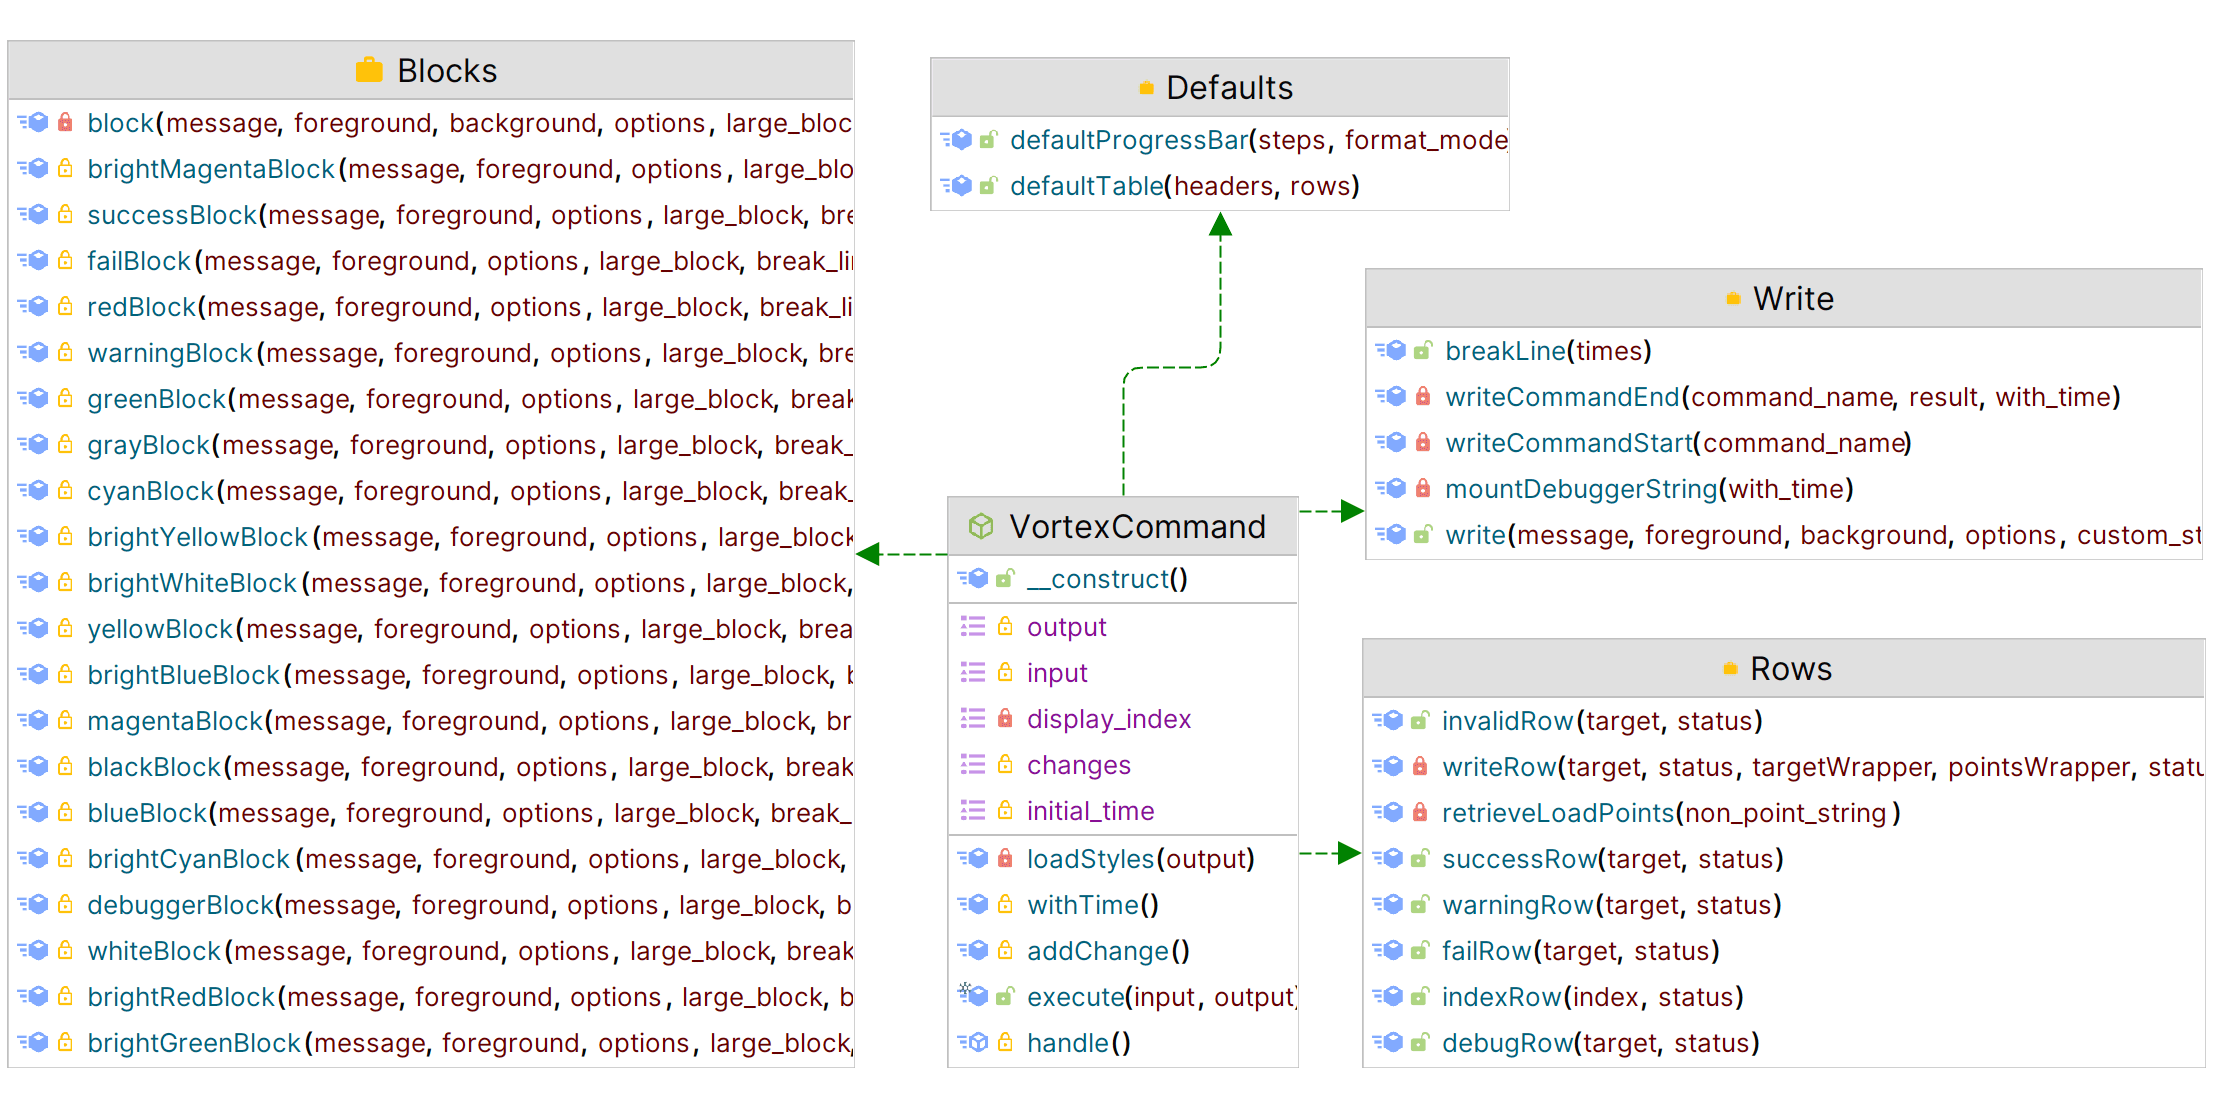
\includegraphics[width=1.0\linewidth]{figures/01_VortexCommandSetup.png}
    \caption{Classe abstrata de comandos e suas classes satélites}
    \label{fig:01_VortexCommandSetup}
\end{figure}

 A figura \ref{fig:01_VortexCommandSetup} representa o grupo de classes responsáveis pela criação de comando tanto no Vortex quanto em uma aplicação que utilize o \textit{framework}.

 \begin{enumerate}
     \item \textbf{VortexCommand.} Classe abstrata que deve ser estendida para criação de comandos personalizados. Esta classe utiliza as \textit{traits}:  \textit{Write}, \textit{Blocks}, \textit{Defaults} e \textit{Rows}. 
     \item \textbf{Defaults.} \textit{Trait} com \textit{layouts default} de tabelas e de barras de progressão para comandos.
     \item \textbf{Blocks.} \textit{Trait} com comandos para estilização de blocos personalizados para criação de comandos.
     \item \textbf{Write.} \textit{Trait} com as opções de escrita para linha de comando disponíveis no Vortex. 
     \item \textbf{Rows.} \textit{Trait} com métodos para criação de linhas formatadas em comandos.
     \item \textbf{OutputStyle.} \textit{Adapter} para receber uma cor de \textit{background} e de \textit{foreground} para escrita em comandos. 
     \item \textbf{\{color\}Output.} Classes para definição de padrões de cores utilizados pelo Cosmo (interface de linha de comando do Vortex).
     \item \textbf{StringWrapper.} \textit{Facade} para simplicação da personalização de textos em comandos da CLI.
 \end{enumerate}

\section{Comandos de interação com a base de dados}

\begin{figure}[H]
    \centering
    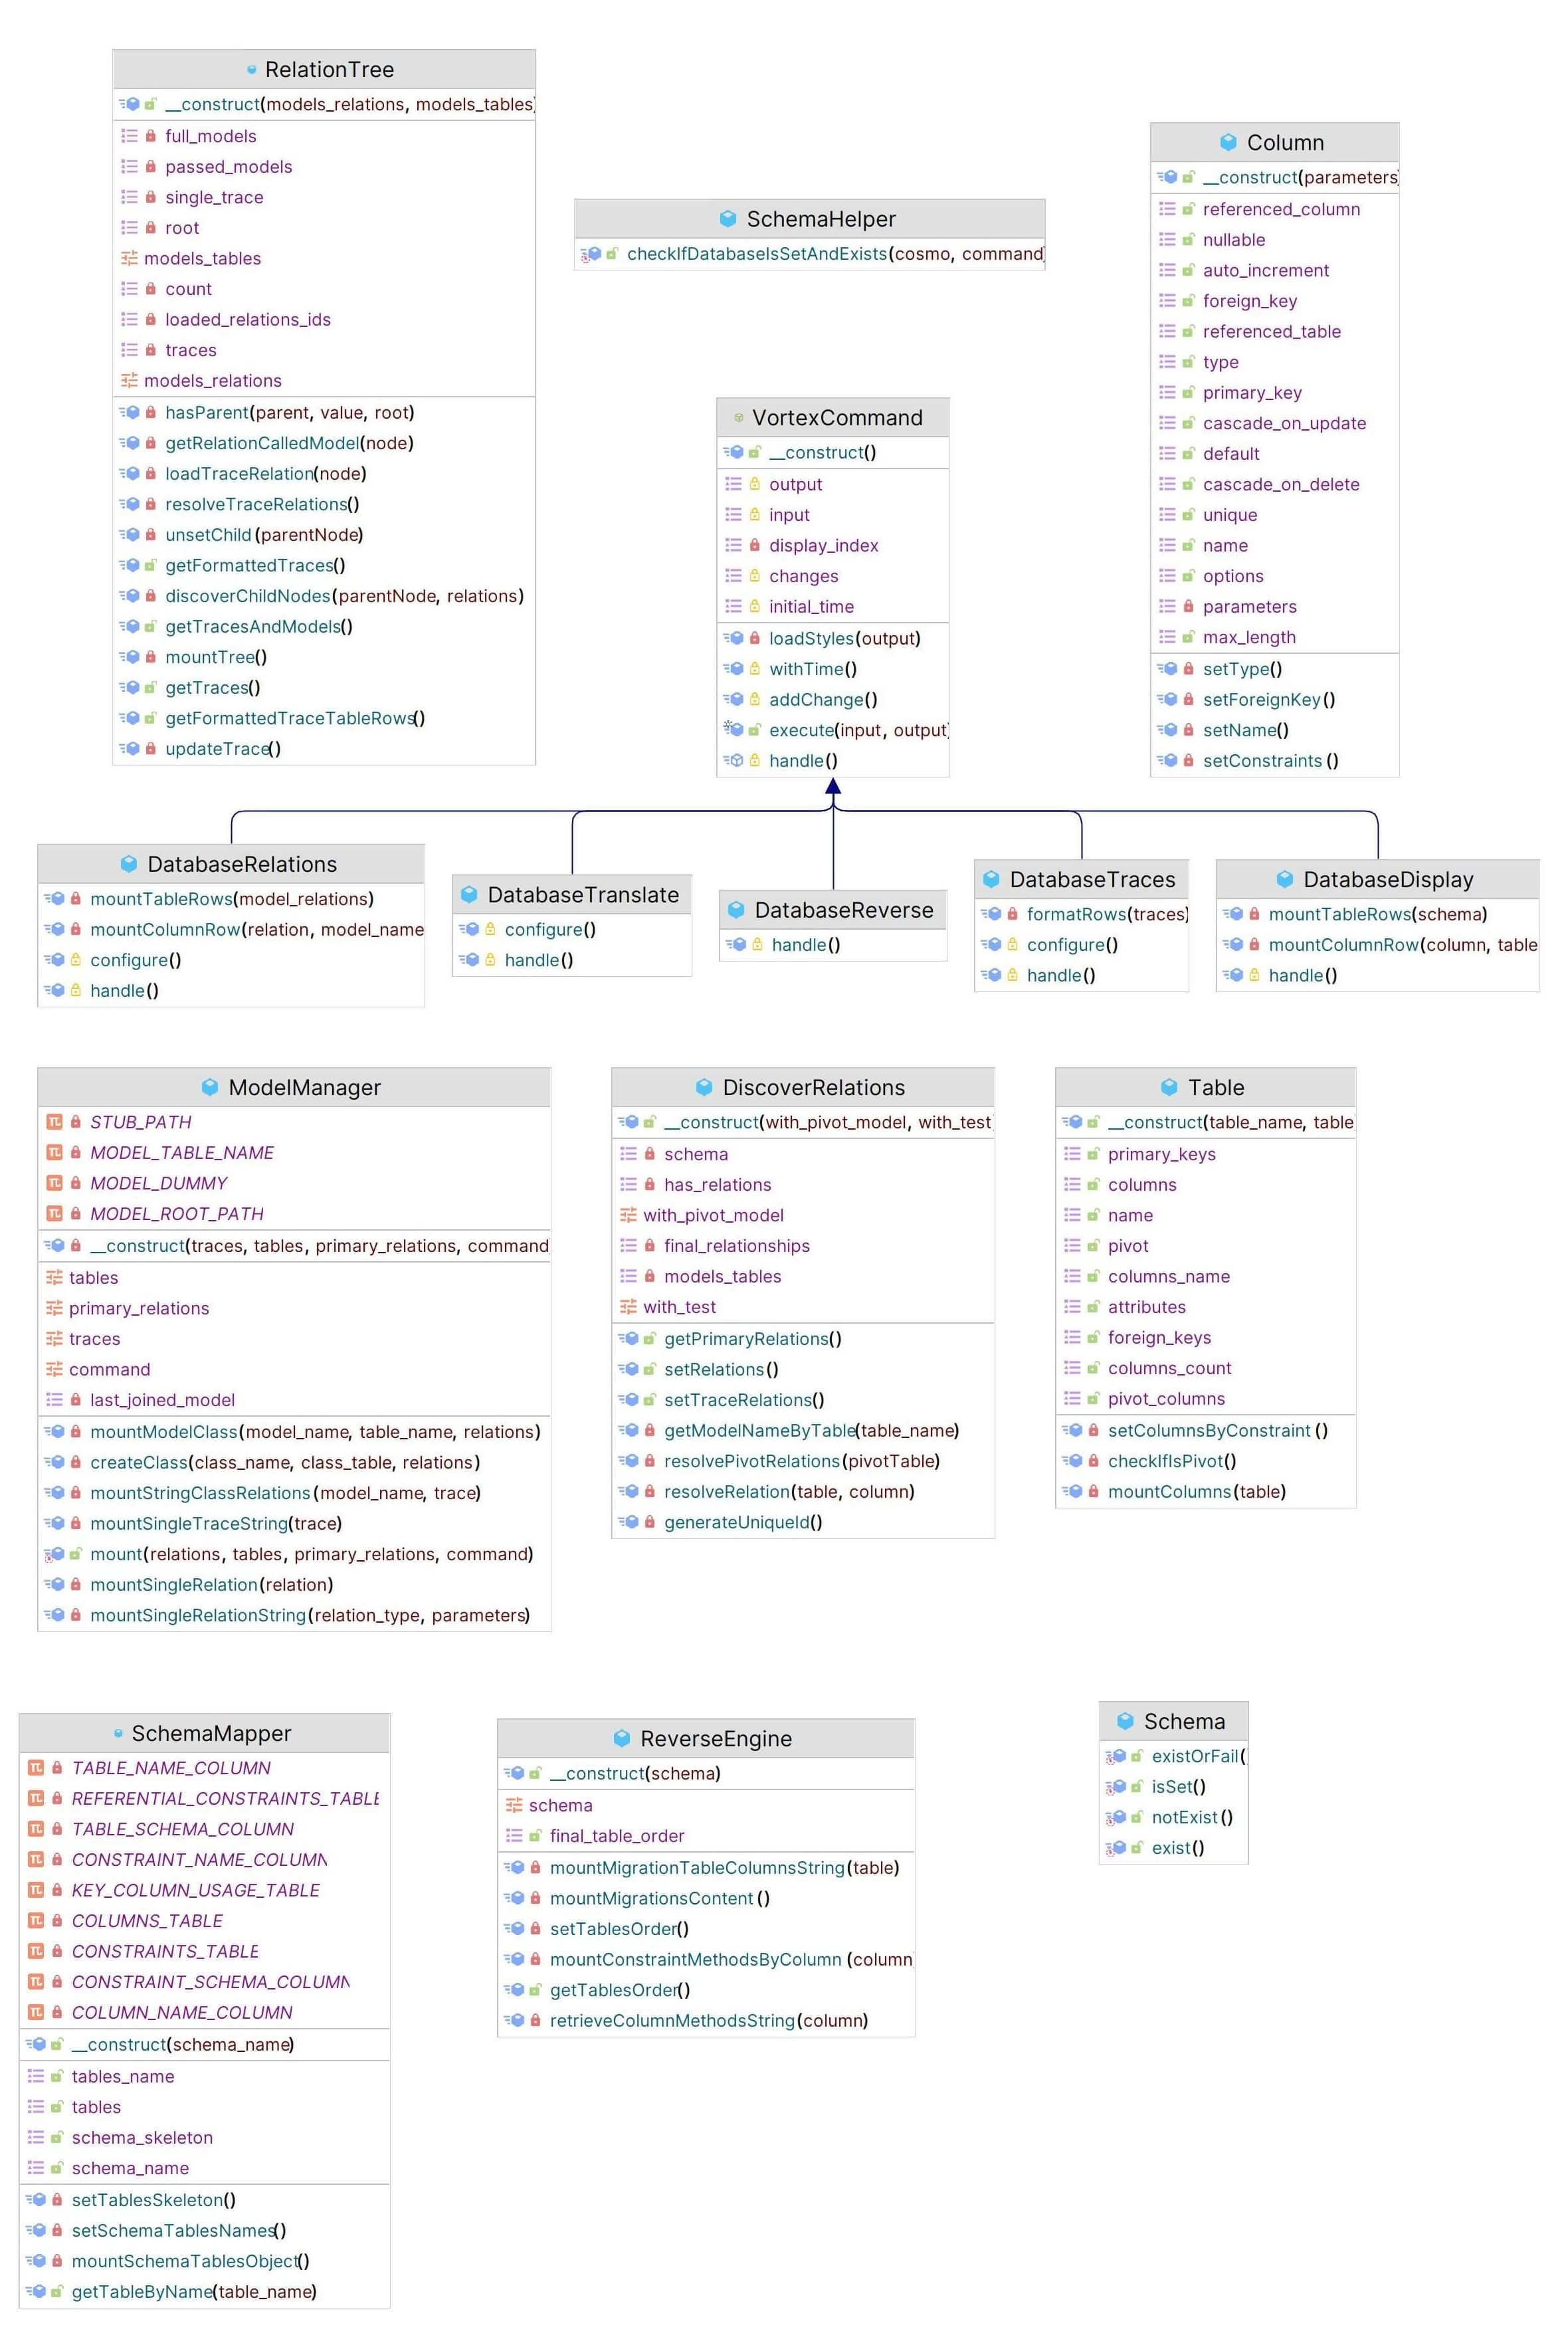
\includegraphics[width=0.9\linewidth]{figures/02_cosmo_commands_database.jpg}
    \caption{Comandos de interação com a base de dados}
    \label{fig:02_cosmo_commands_database}
\end{figure}

 A figura \ref{fig:02_cosmo_commands_database} agrupa os comandos responsáveis por interações com a base de dados, sendo que tais interações não alteram a estrutura e nem o estado da base de dados. Além destes comandos estão presentes classes que realizam o mapeamento da estrutura da base de dados e a tradução da mesma para \textit{scripts} PHP.

 \begin{enumerate}
     \item \textbf{DatabaseRelations.} Classe que representa o comando para dar \textit{print} nos relacionamnetos da base de dados relacional.
     \item \textbf{DatabaseTranslate.} Classe que realiza o comando para tradução da base de dados em classes modelo com relacionamentos.
     \item \textbf{DatabaseReverse.} Comando que realiza a engenharia reversa da base de dados em migrações.
     \item \textbf{DatabaseTraces.} Classe que realiza o \textit{print} de todos os relacionamentos do tipo \textit{trace} da base de dados.
     \item \textbf{DatabaseDisplay.} Comando para obter a representação das tabelas da base de dados.
     \item \textbf{SchemaMapper.} Classe que realiza o mapeamento das tabelas da base de dados juntamente com seus relacionamentos.
     \item \textbf{Schema.} Classe que recebe os dados do \textit{schema} da base de dados da aplicação.
     \item \textbf{Table.} Classe que armazena os dados de uma tabela da base de dados.
     \item \textbf{Column.} Classe que armazena os dados de uma coluna da base de dados.
     \item \textbf{ReverseEngine.} Classe que realiza o mapeamento das migrações a partir o \textit{schema} da base de dados, utilizado juntamente com o comando \textit{database:reverse}.
     \item \textbf{DiscoverRelations} Classe que realiza o mapeamento dos relacionamentos primários da base de dados e a partir destes a partir de uma estrutura de árvore binária para mapear os \textit{trace relations}.
     \item \textbf{ModelManager.} Classe que extrai os modelos a partir dos relacionamentos e cria os mesmos na aplicação.
 \end{enumerate}

\section{Comandos de criação de classes da arquitetura do \textit{framework}}

\begin{figure}[H]
    \centering
    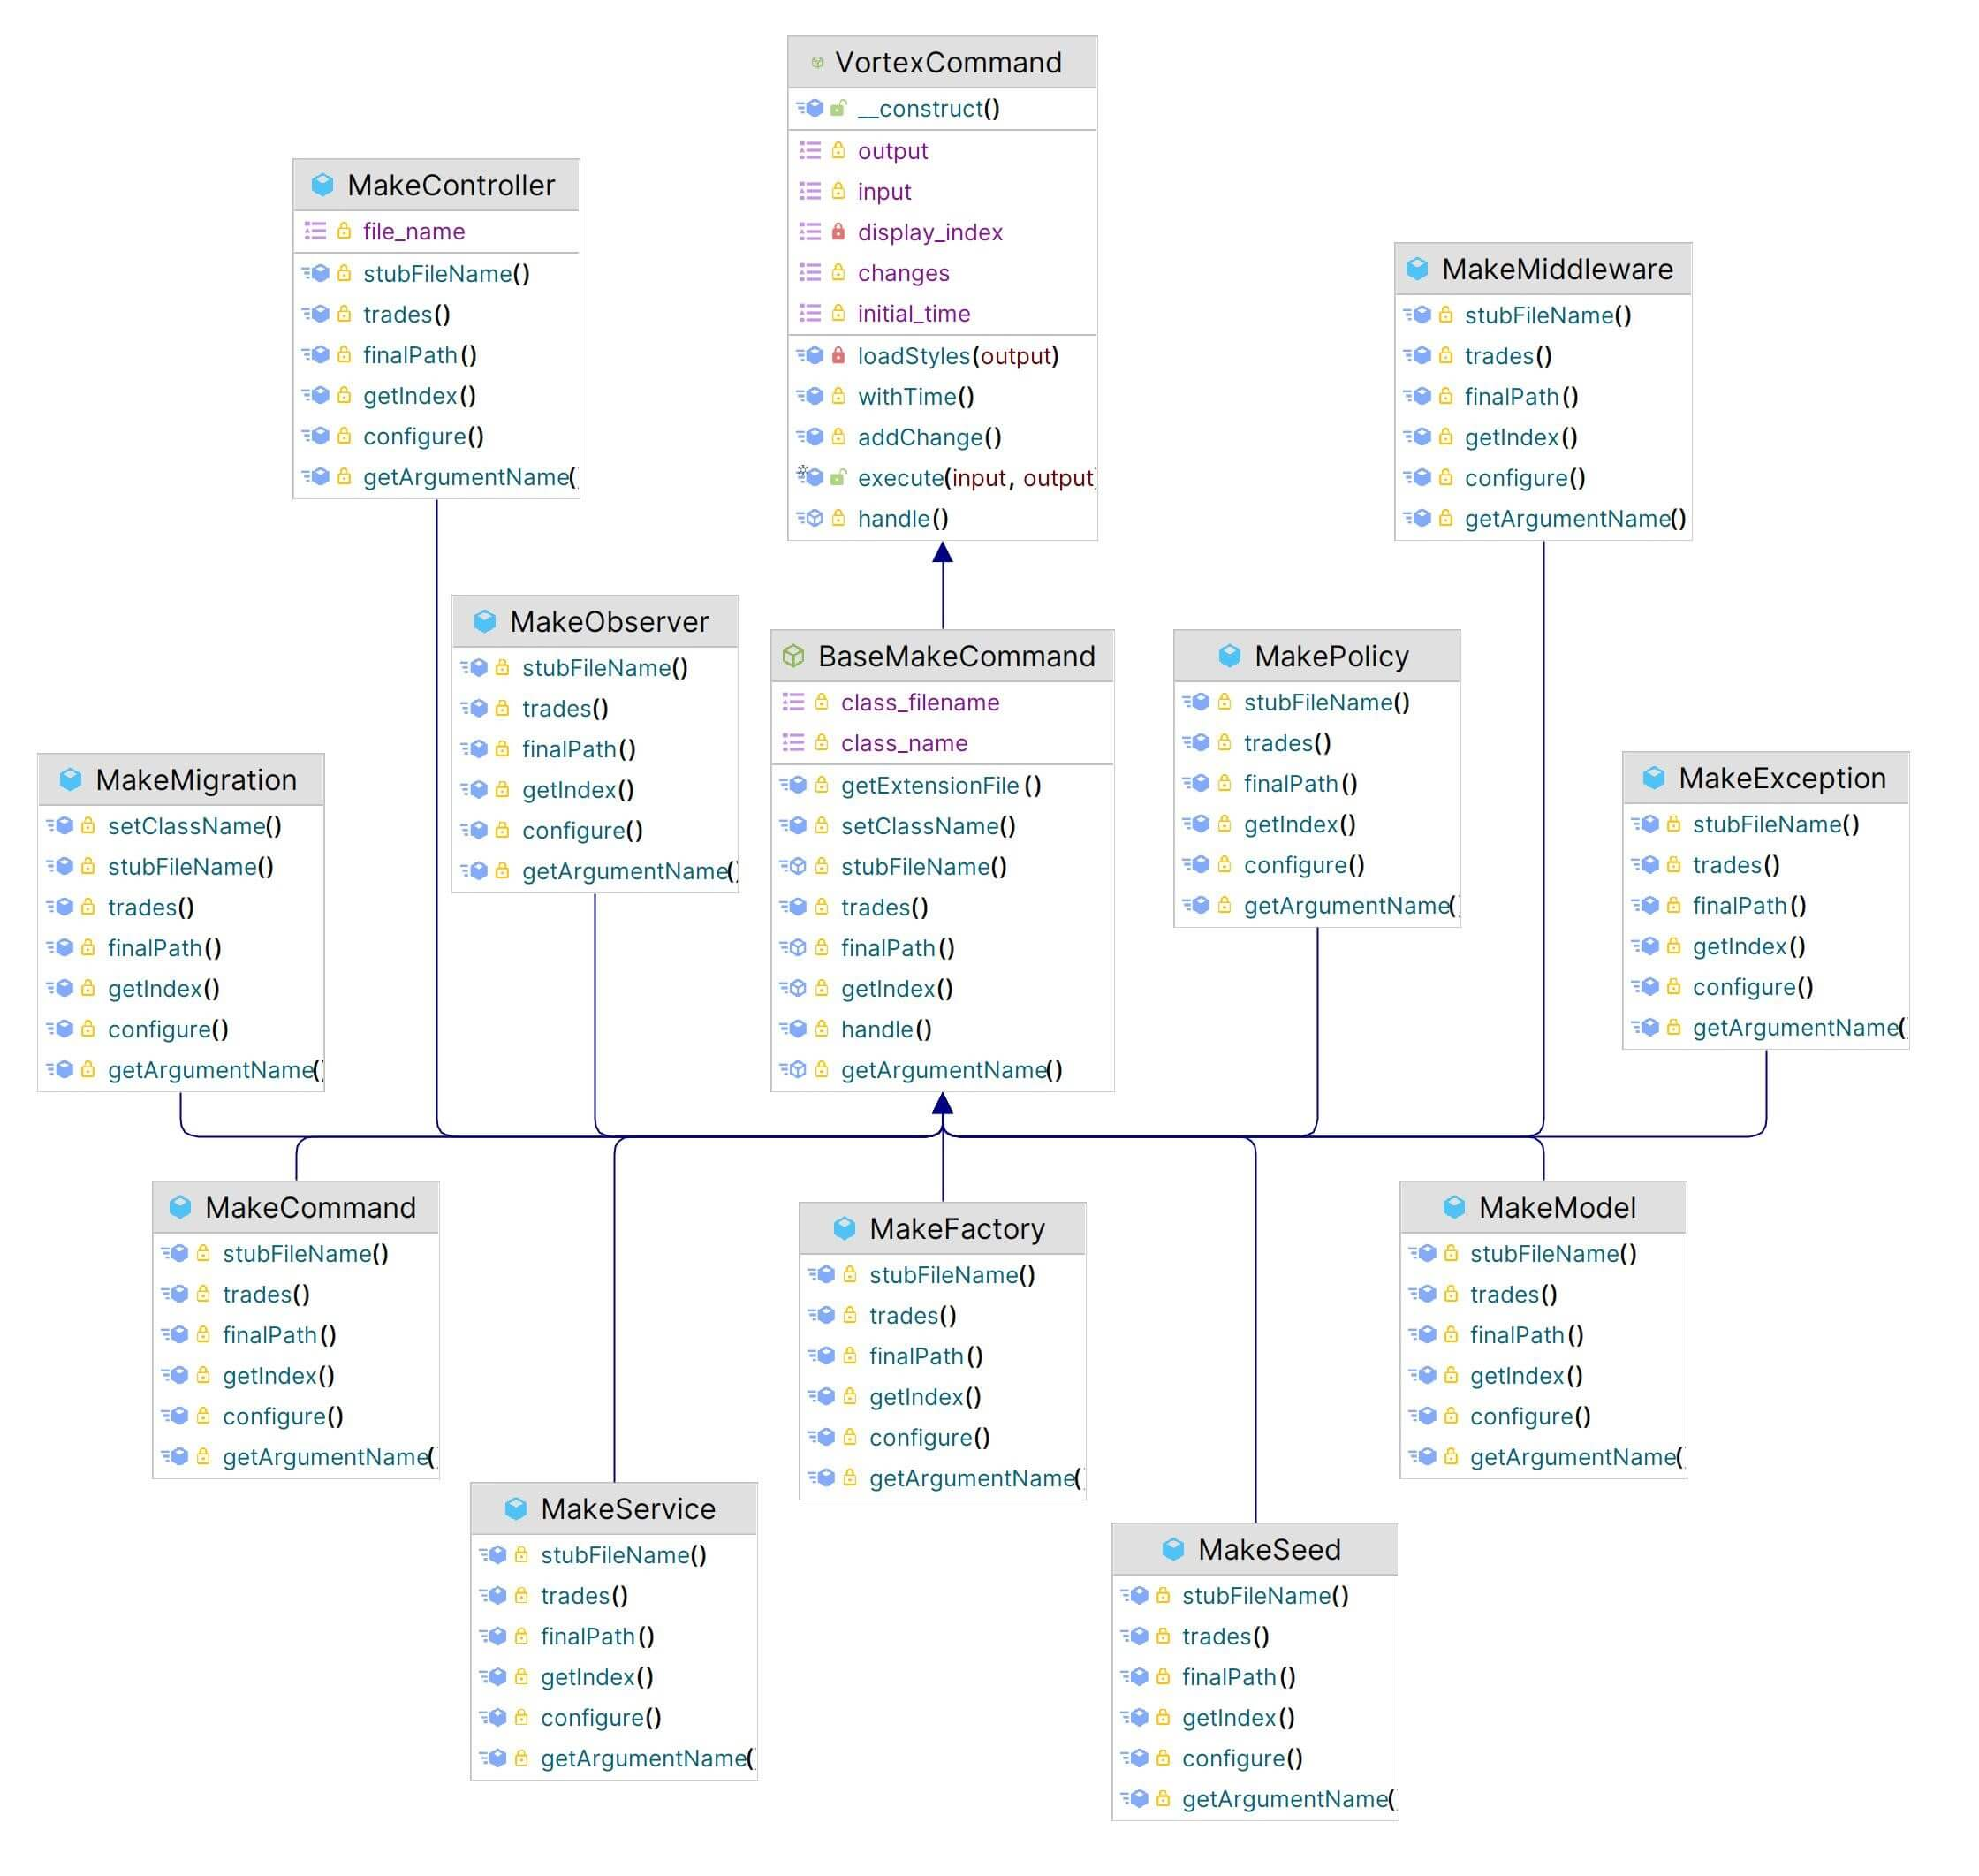
\includegraphics[width=0.9\linewidth]{figures/03_cosmo_commands_make.jpg}
    \caption{Classes de comandos para criação de classes especificas da arquitetura do \textit{framework}}
    \label{fig:03_cosmo_commands_make}
\end{figure}

 Na figura \ref{fig:03_cosmo_commands_make} temos a abstração do Vortex responsável pela criação de classes importantes para o devido funcionamento de uma aplicação no \textit{framework}.

 \begin{enumerate}
     \item \textbf{BaseMakeCommand.} Classe abstrata base para criação de comandos que criam classes especificas do \textit{framework}, como modelos, migrações, entre outras.
     \item \textbf{Make\{class\}.} Classes comando que estendem de BaseMakeCommand e representam a criação de uma das diversas classes que podem ser criadas pela linha de comando.
 \end{enumerate}

 \section{Classes de comandos \textit{uncategorized}}

\begin{figure}[H]
    \centering
    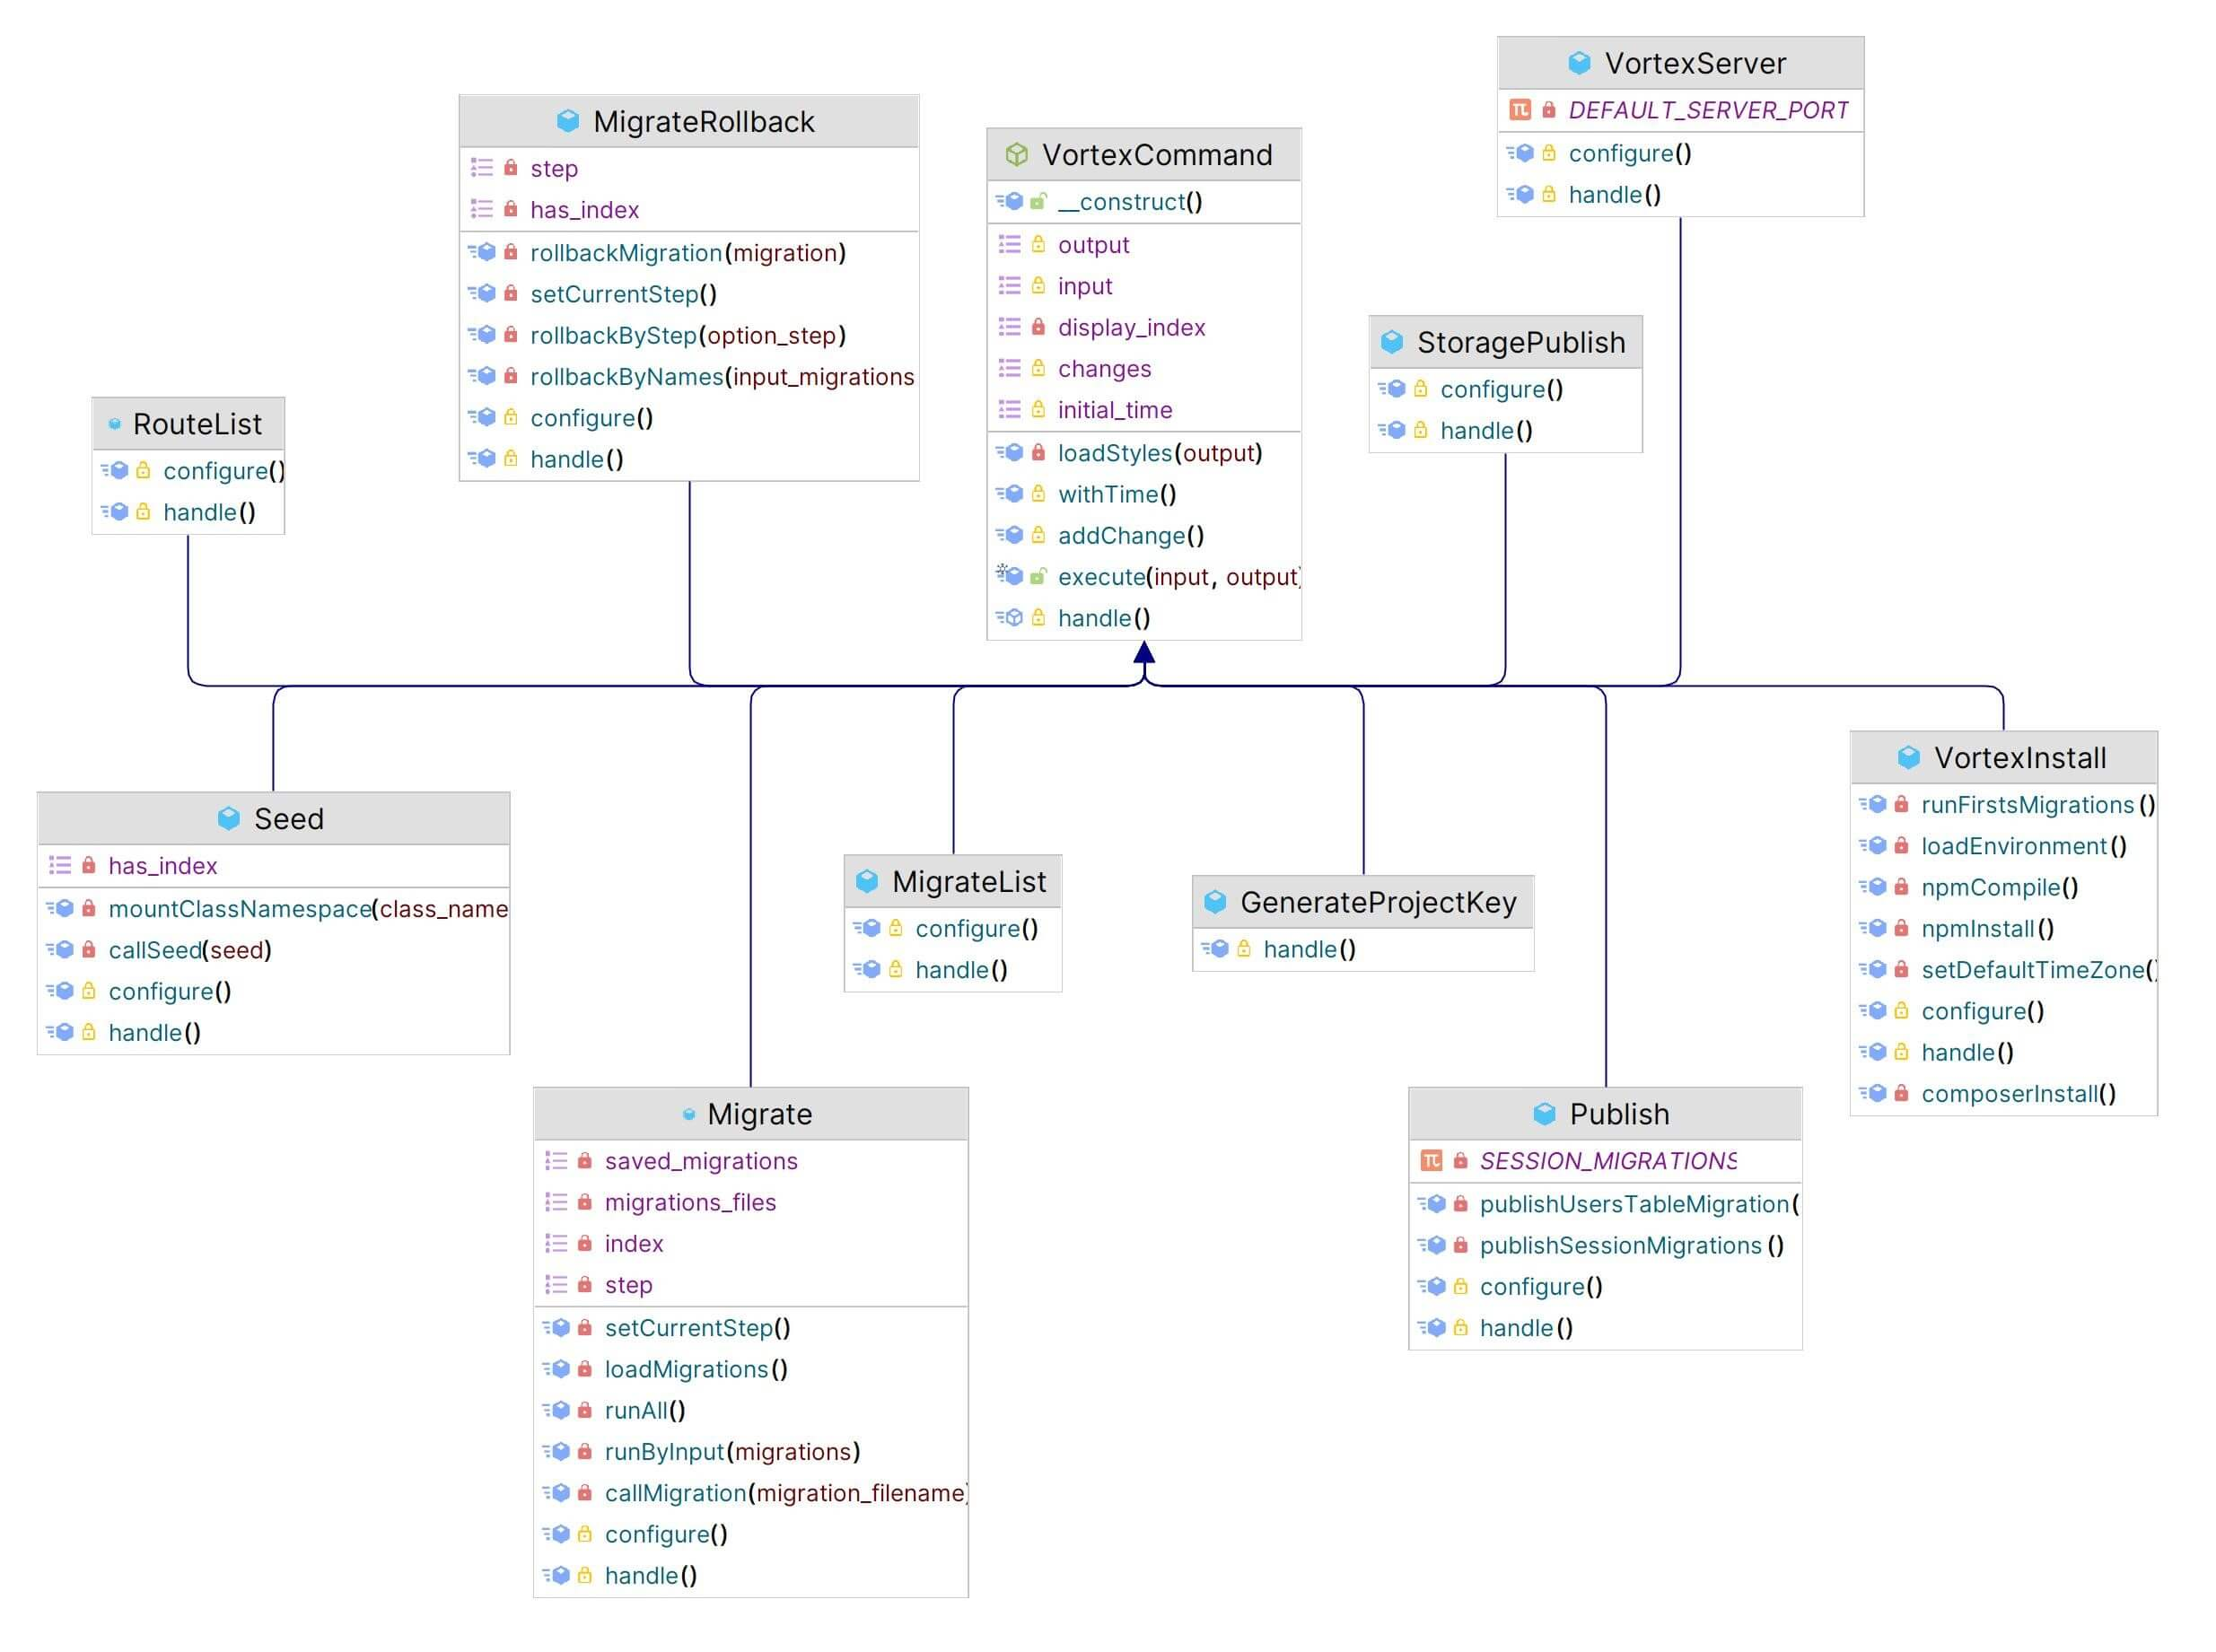
\includegraphics[width=0.9\linewidth]{figures/04_cosmo_commands_uncategoryzed.jpg}
    \caption{Classes de comandos \textit{uncategorized}}
    \label{fig:04_cosmo_commands_uncategoryzed}
\end{figure}

 \begin{enumerate}
     \item \textbf{Migrate.} Classe comando que realiza a execução das migrações da aplicação baseando-se ou em parâmetros de nome de migrações passados por parâemtro ou por um \textit{step}, que pode ser passado juntamente do comando ou serão executadas todas as migrações que não foram executadas.
     \item \textbf{MigrateList.} Classe que realiza o \textit{print} de todas as migrações da aplicação na linha de comando.
     \item \textbf{MigrateRollback.} Comando que pode receber o nome de uma migração ou um \textit{step} para realização o método \textit{down} de tais migrações, caso nenhum parâmetro seja passado, serão executados os métodos das migrações com o último \textit{step} da base de dados.
     \item \textbf{RouteList.} Classe que retornará a lista com todas as rotas da aplicação, incluindo informações como método HTTP, controladora e método responsável por tal rota.
     \item \textbf{VortexInstall.} Classe que realiza a instalação inicial das dependências da aplicação.
     \item \textbf{VortexServer.} Comando que executa o servidor embutido do PHP.
     \item \textbf{Seed.} Classe comando que executa as classes \textit{seeds} que realizam inserções na base de dados, caso receba um parâmetro válido para nome de classe, apenas esta será executada, caso nenhum parâmetro for inserido, todas as classes \textit{seeds} serão executadas.
     \item \textbf{Publish.} Comando para publicação de recursos do \textit{framework}.
     \item \textbf{GenerateProjectKey.} A chave única do projeto fica armazenada no arquivo de variáveis de ambiente (.env) na raiz do projeto. Esta classe quando executada pela CLI gera aleatoriamente e armazena ou troca a chave única da aplicação.
     \item \textbf{StoragePublish.} Classe que cria o \textit{link} simbólico para o \textit{storage}.
 \end{enumerate}

\section{\textit{Observers} e \textit{Policies}}

\begin{figure}[H]
    \centering
    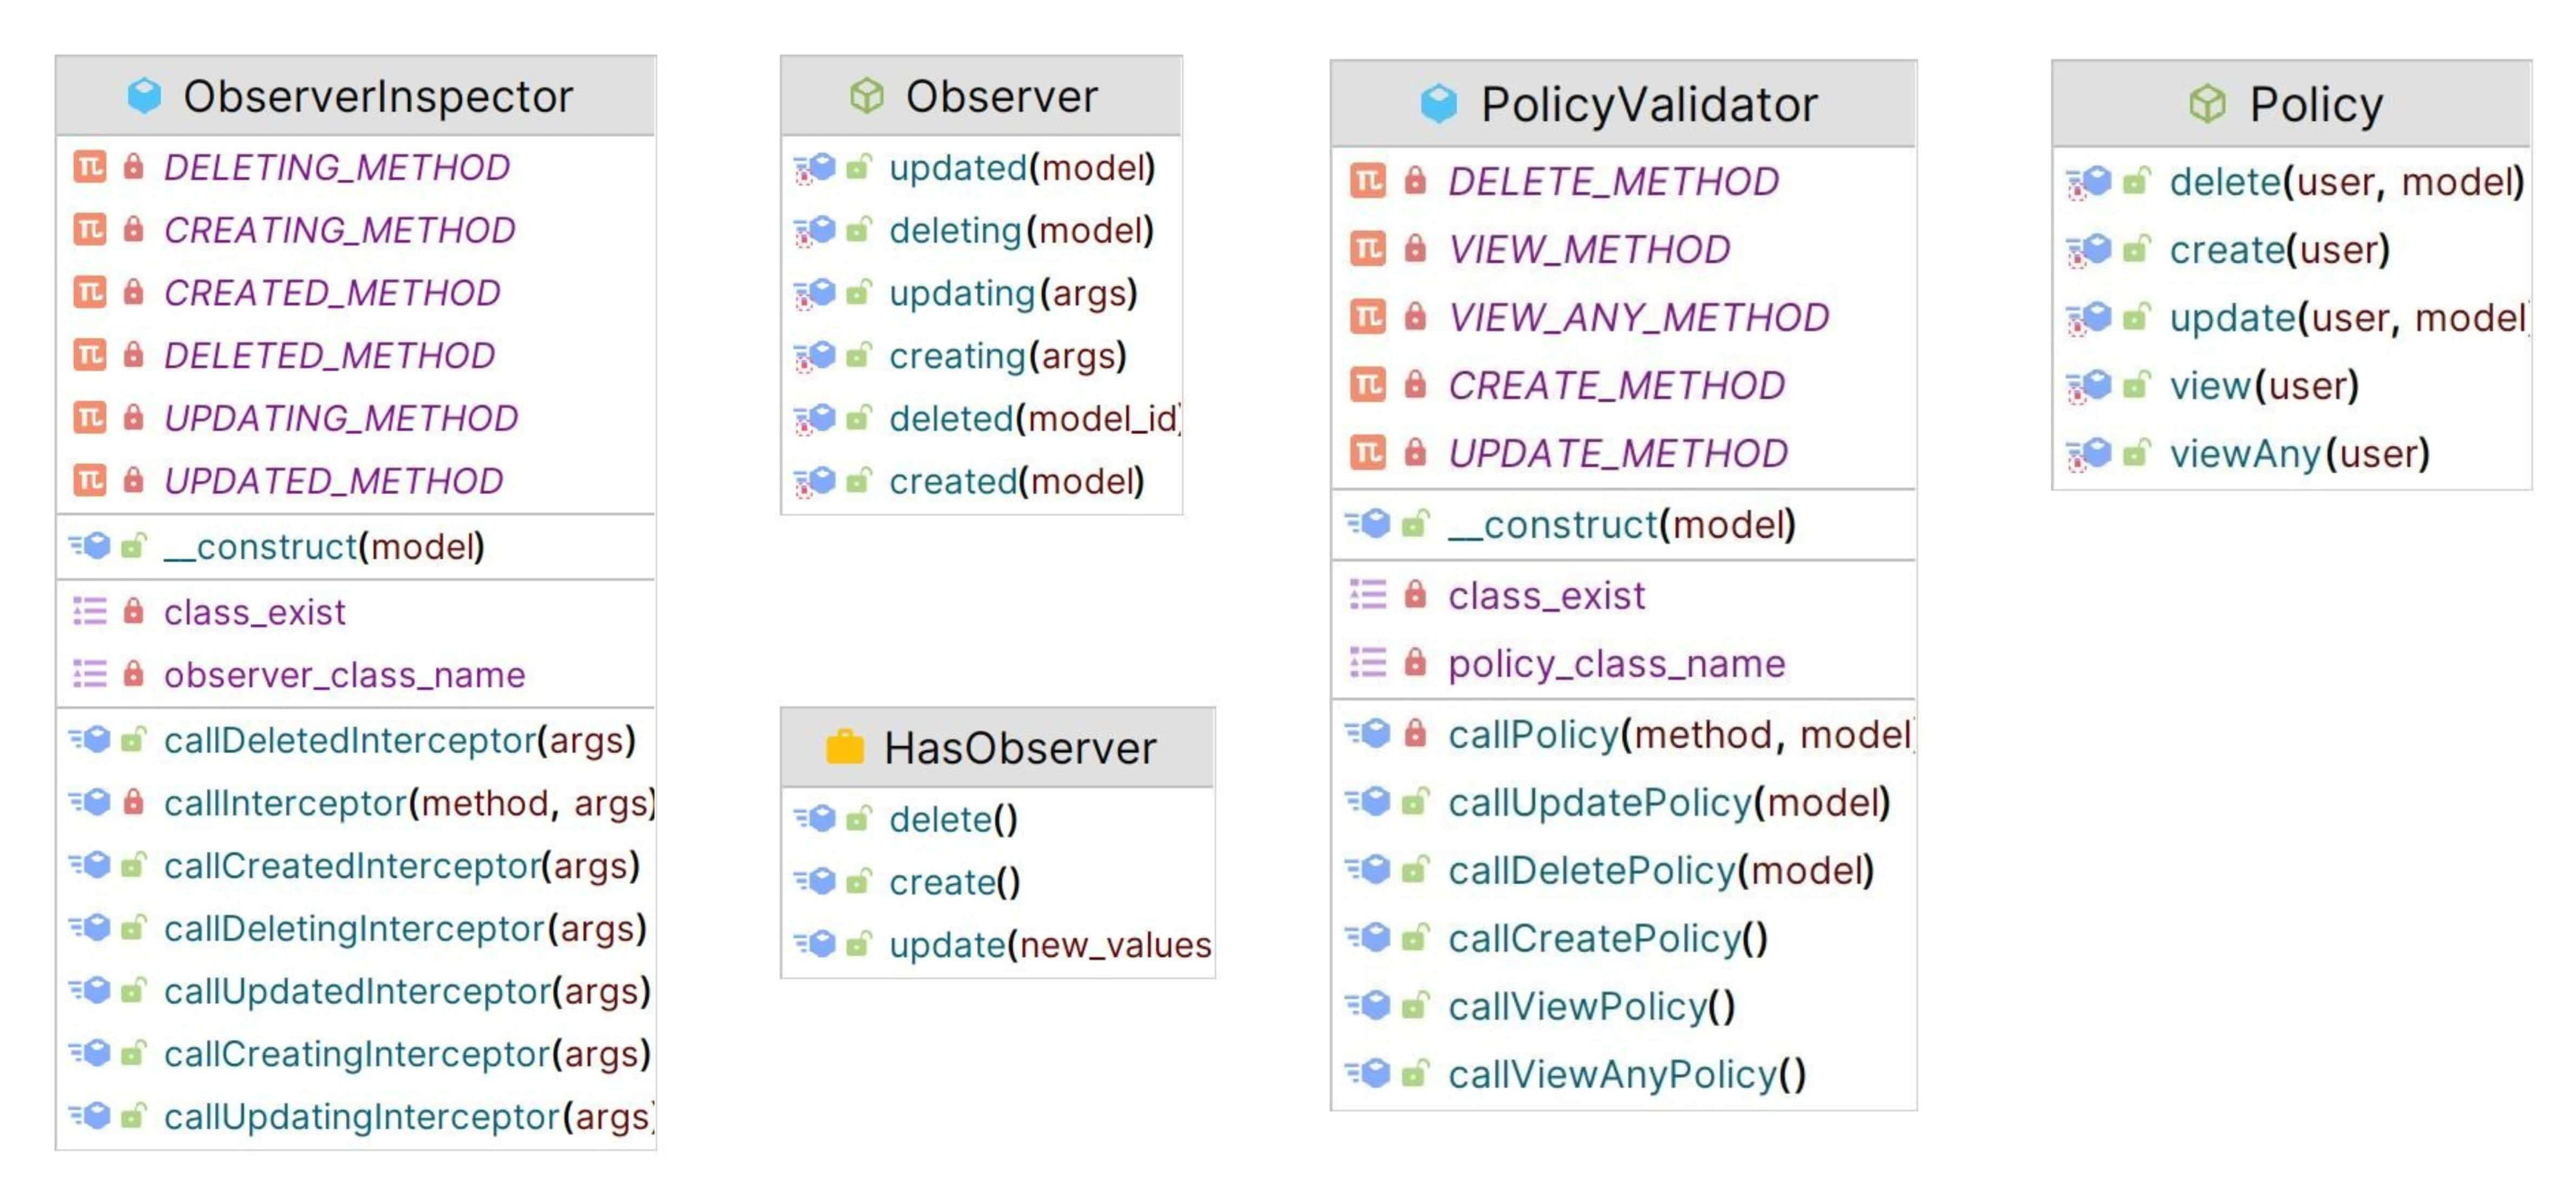
\includegraphics[width=0.9\linewidth]{figures/05_observer_policy.jpg}
    \caption{Classes de \textit{observers} e \textit{policies}}
    \label{fig:05_observer_policy}
\end{figure}

 Na figura \ref{fig:05_observer_policy} temos a abstração de \textit{observers} e \textit{policies}, que estão diretamente relacionadas as classes modelos nas aplicações, tendo em vista que cada \textit{observer} e \textit{policy} deve ser associado a uma classe modelo.

 \begin{enumerate}
     \item \textbf{Observer.} Classe abstrata base para criação de \textit{observers} que quando associados a uma classe modelo permitem a execução de rotinas de \textit{script} em momentos específicos do manejamento de modelos, como: antes da criação de um objeto modelo, após a criação, antes da exclusão de um modelo e entre outros.
     \item \textbf{HasObserver.} \textit{Trait} responsável por alterar os métodos base de modelos que possuem \textit{observer}, essa \textit{trait} deve ser utilizada pela classe modelo.
     \item  \textbf{ObserverInspector.} Classe responsável por executar os \textit{scripts} determinados pelos \textit{observers}.
     \item \textbf{Policy.} Classe abstrata que quando associada corretamente a uma classe modelo permite validar a permissão para realizar determinada operação com um objeto modelo.
     \item \textbf{PolicyValidator.} Classe que valida a execução de determinado \textit{script} de acordo com as definições da classe \textit{policy}.
 \end{enumerate}

 \section{Controladores de requisição e sessão}

\begin{figure}[H]
    \centering
    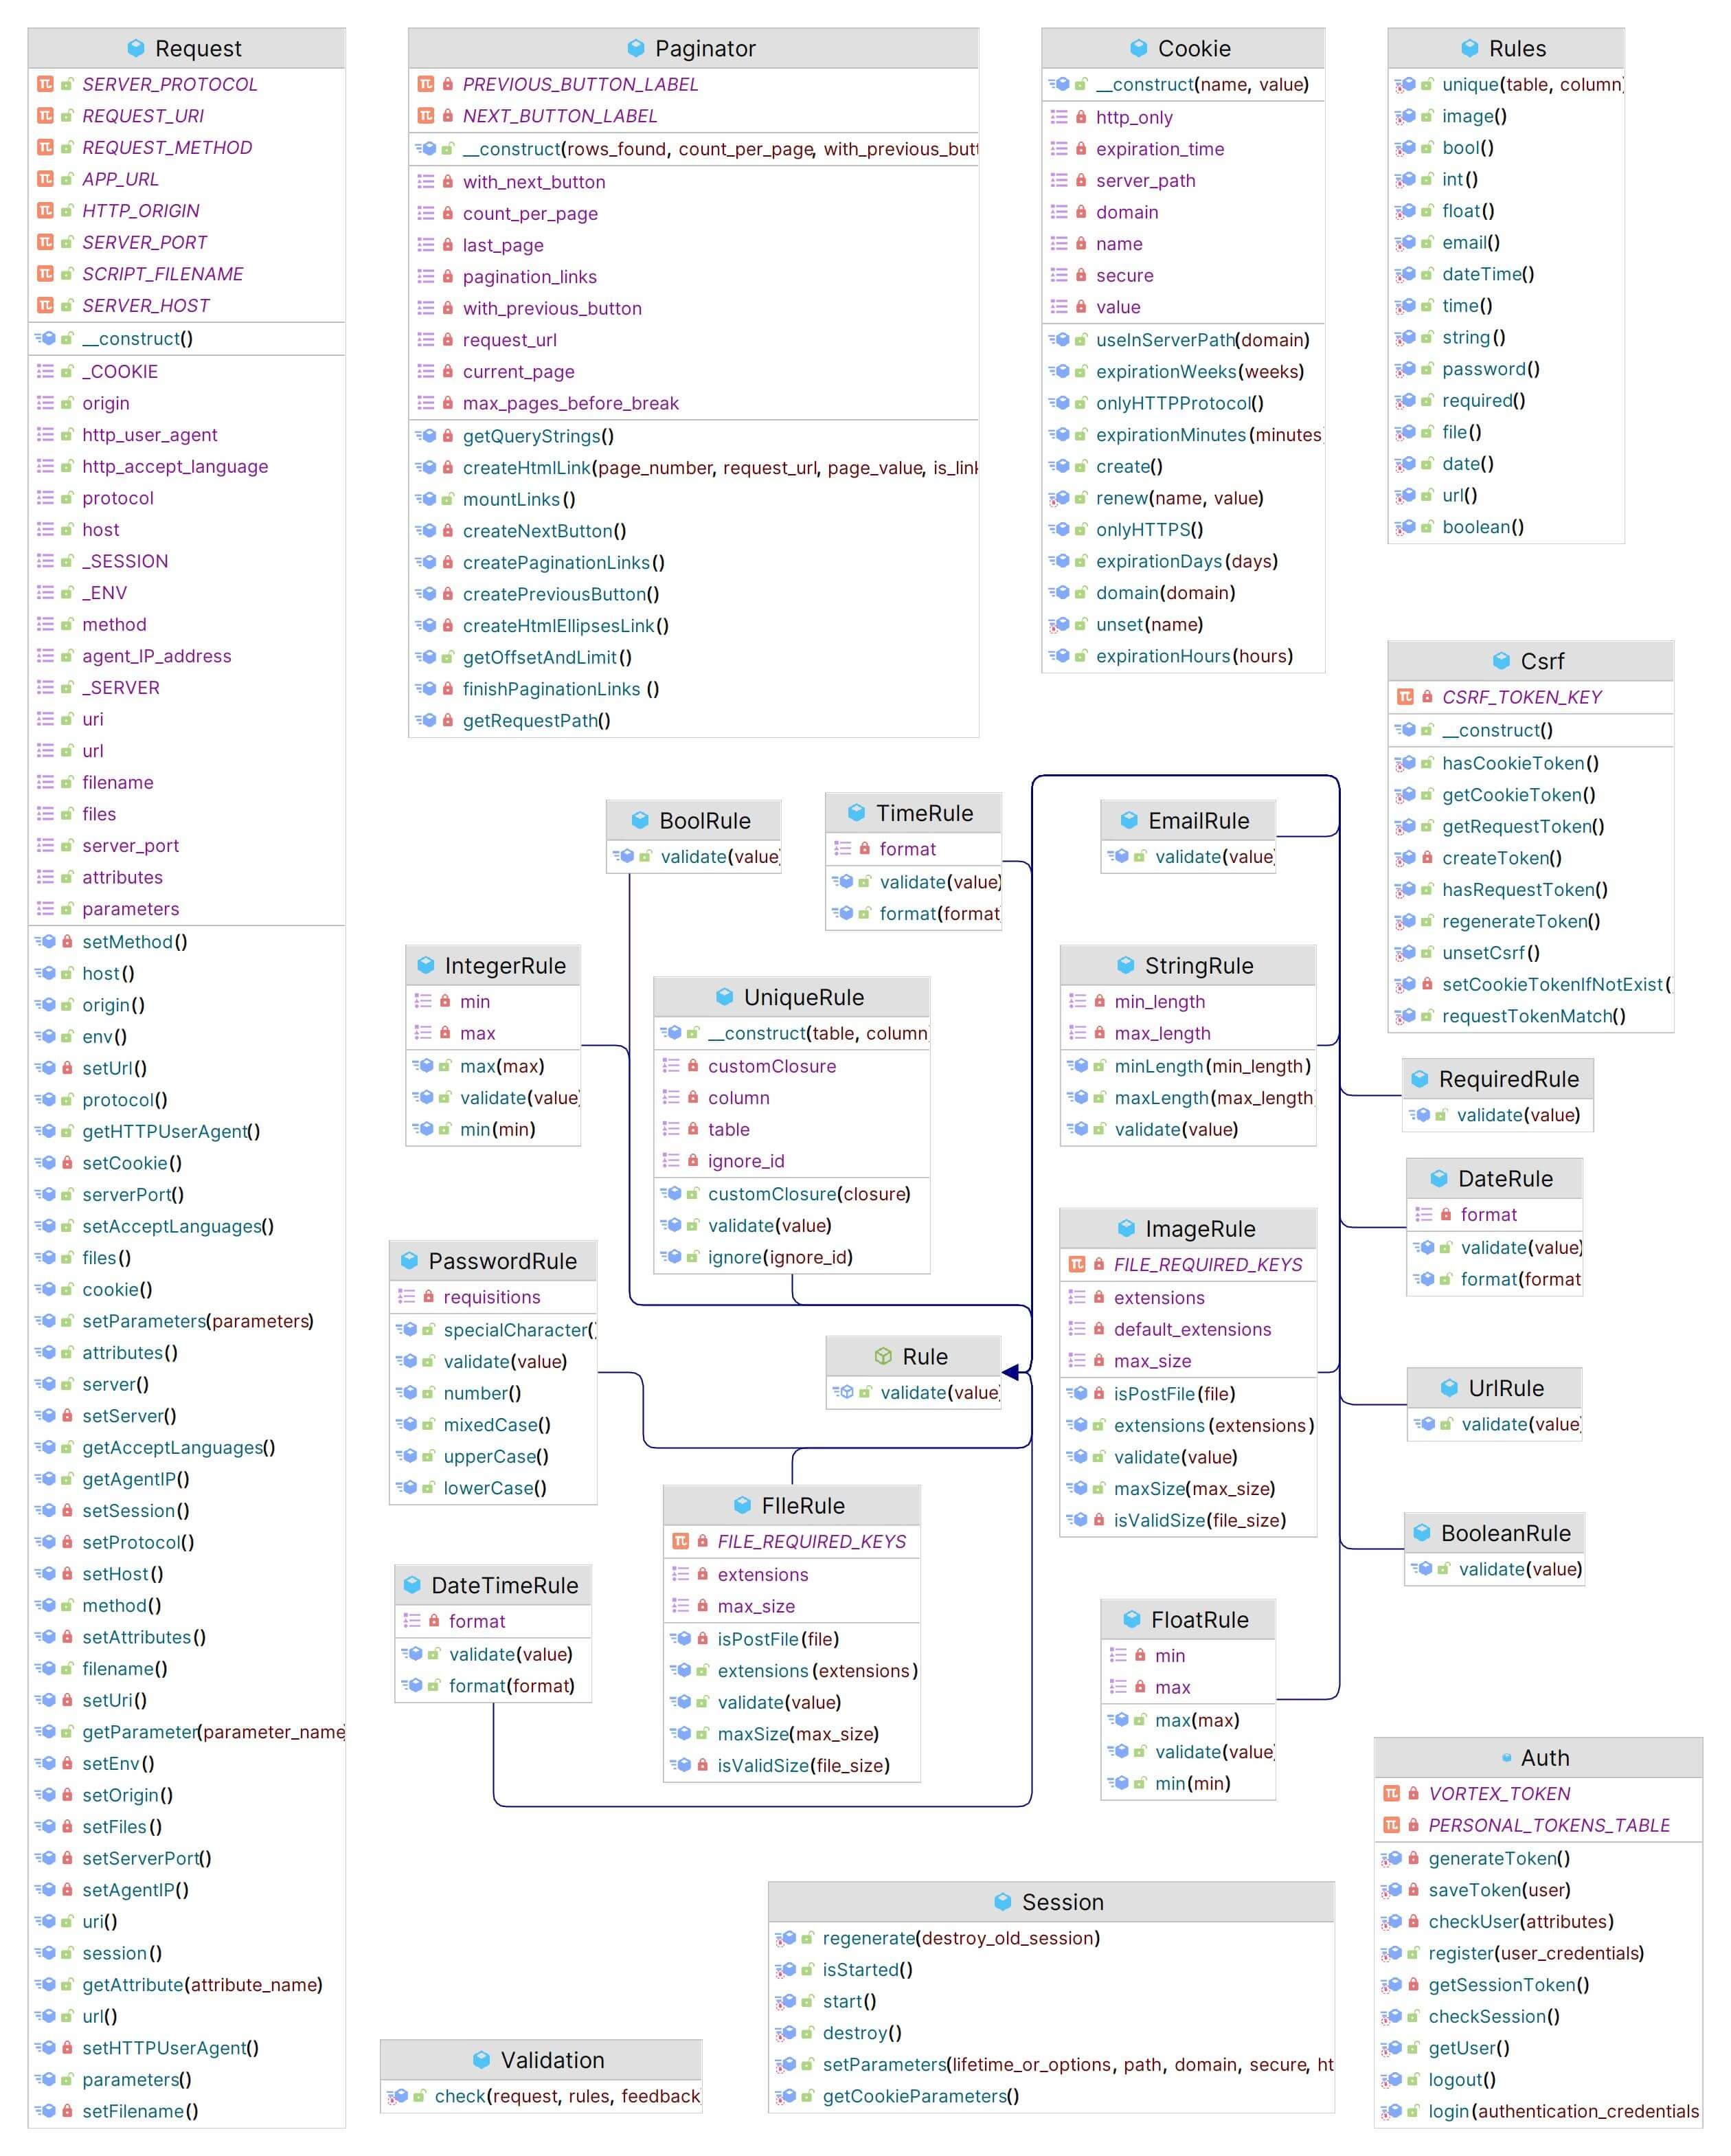
\includegraphics[width=1.0\linewidth]{figures/08_request_auth.jpg}
    \caption{Classes de \textit{observers} e \textit{policies}}
    \label{fig:08_request_auth}
\end{figure}

De acordo com a \ref{fig:08_request_auth} tem-se que as diversas classes apresentadas são responsáveis por controlar ou validar os dados da requisição ou da sessão, incluindo \textit{cookies} e validadores de requisição.

 \begin{enumerate}
     \item \textbf{Request.} Classe que abstrai todas as informações presentes na requisição, sendo embutida em rotas do tipo POST da aplicação e podendo ser acessada globalmente.
     \item \textbf{Paginator.} Permite realizar a paginação de consultas diretamente pelo ORM. Possui métodos que permitem escolher o número de registros por página, a página atual e intervalo de quebra de páginas.
     \item \textbf{Cookie.} Classe para manejamento de dados de \textit{cookies}.
     \item \textbf{Rules.} Classe para acesso as regras de validação nativas do \textit{framework}.
     \item \textbf{\{type\}Rule.} Classe abstrata base para criação de regras de validação.
     \item \textbf{Validation.} Classe que realiza a validação da requisição com as regras passadas.
     \item \textbf{Session.} Classe para controle de sessão, permitindo criar, alterar, destruir e buscar dados presentes na sessão atual.
     \item \textbf{Auth.} \textit{Helper} para acesso rápido a dados do usuário autenticado.
     \item \textbf{Csrf.} Classe para verificação e validação de \textit{tokens} do tipo CSRF.
 \end{enumerate}

 \section{Interação com arquivos, diretórios e \textit{links} simbólicos}

\begin{figure}[H]
    \centering
    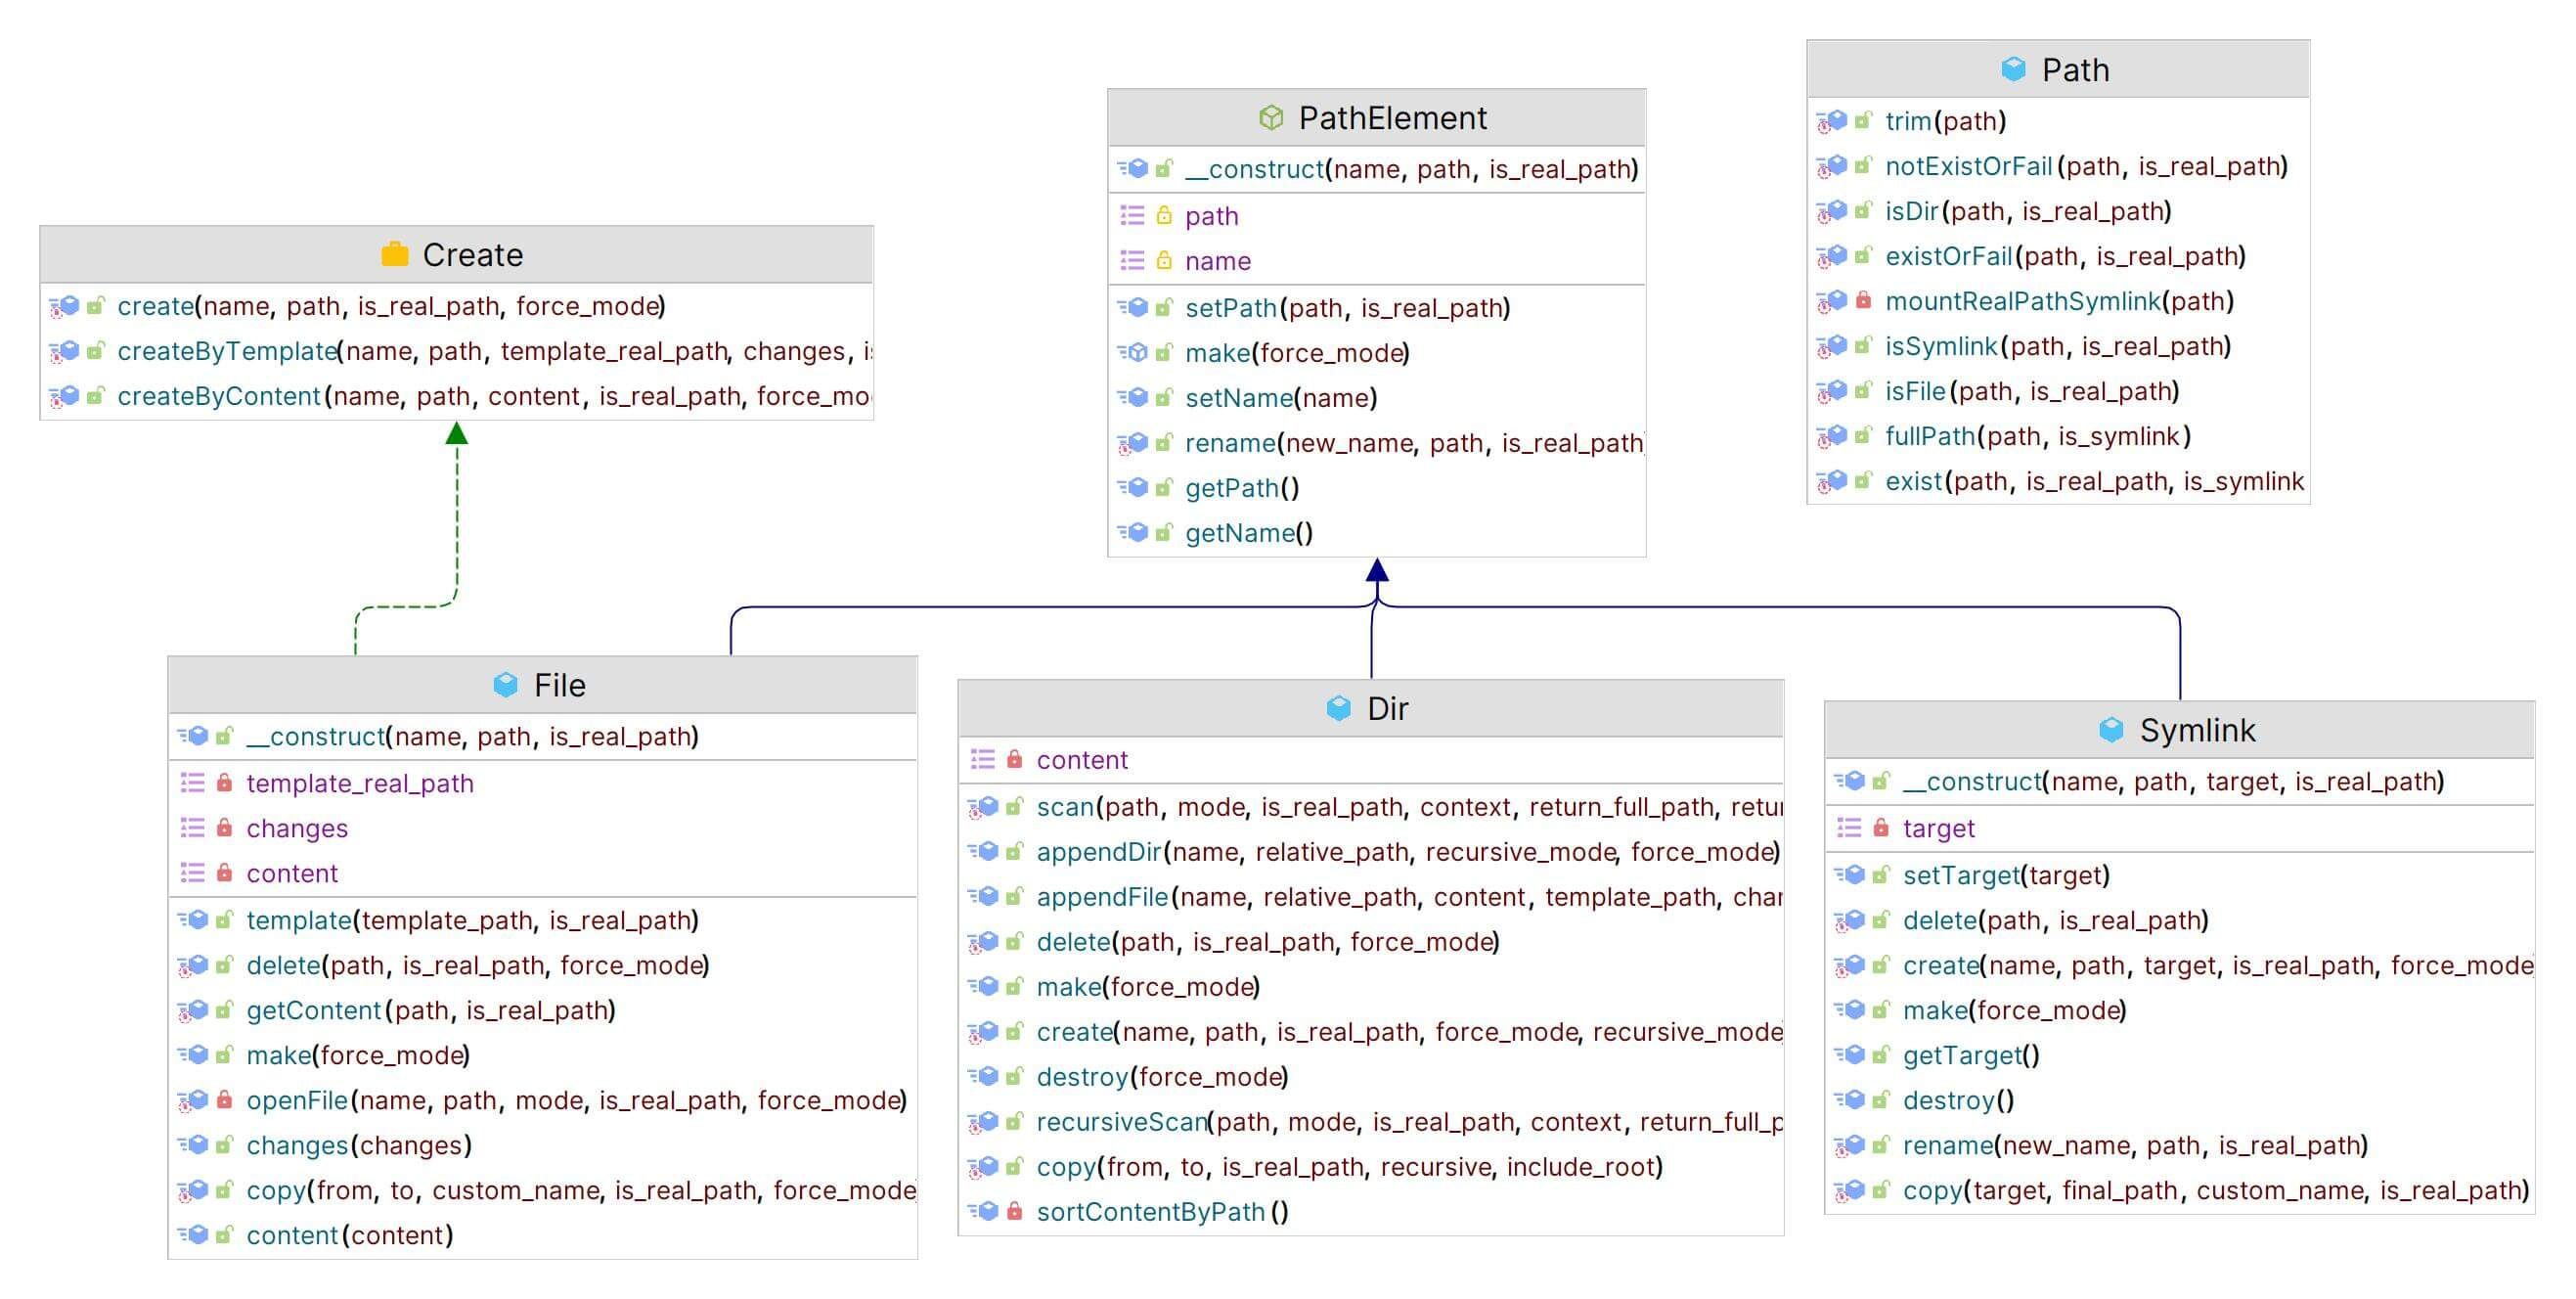
\includegraphics[width=0.9\linewidth]{figures/09_file_directory_manage.jpg}
    \caption{Classes de interação com arquivos, diretórios e \textit{links} simbólicos}
    \label{fig:09_file_directory_manage}
\end{figure}

A figura \ref{fig:09_file_directory_manage} condensa as classes responsáveis por criar, editar, deletar e checar arquivos, diretórios e \textit{links} simbólicos dentro da arquitetura do \textit{framework}.

 \begin{enumerate}
     \item \textbf{PathElement.} Classe abstrata que serve de base para as outras três classes que gerenciam as estruturas de elementos ''físicos'' da aplicação.
     \item \textbf{Dir.} Classe que controla todas as operações com diretórios dentro do \textit{framework}.
     \item \textbf{Path.} \textit{Helper} para acesso rápido as classes de elementos estruturais desta seção.
     \item \textbf{File.} Classe para manejar todas as interações com arquivos dentro do \textit{framework}.
     \item \textbf{Symlink.} Clase que interage com \textit{links} simbólicos dentro da arquitetura do \textit{framework}.
     \item \textbf{Create.} \textit{Trait} para abstração das diversas operações de criação de arquivos, sendo elas: criação baseada em \textit{strings}, baseadas em \textit{template} e cópias de arquivos.
 \end{enumerate}

 \section{Criptografia}

\begin{figure}[H]
    \centering
    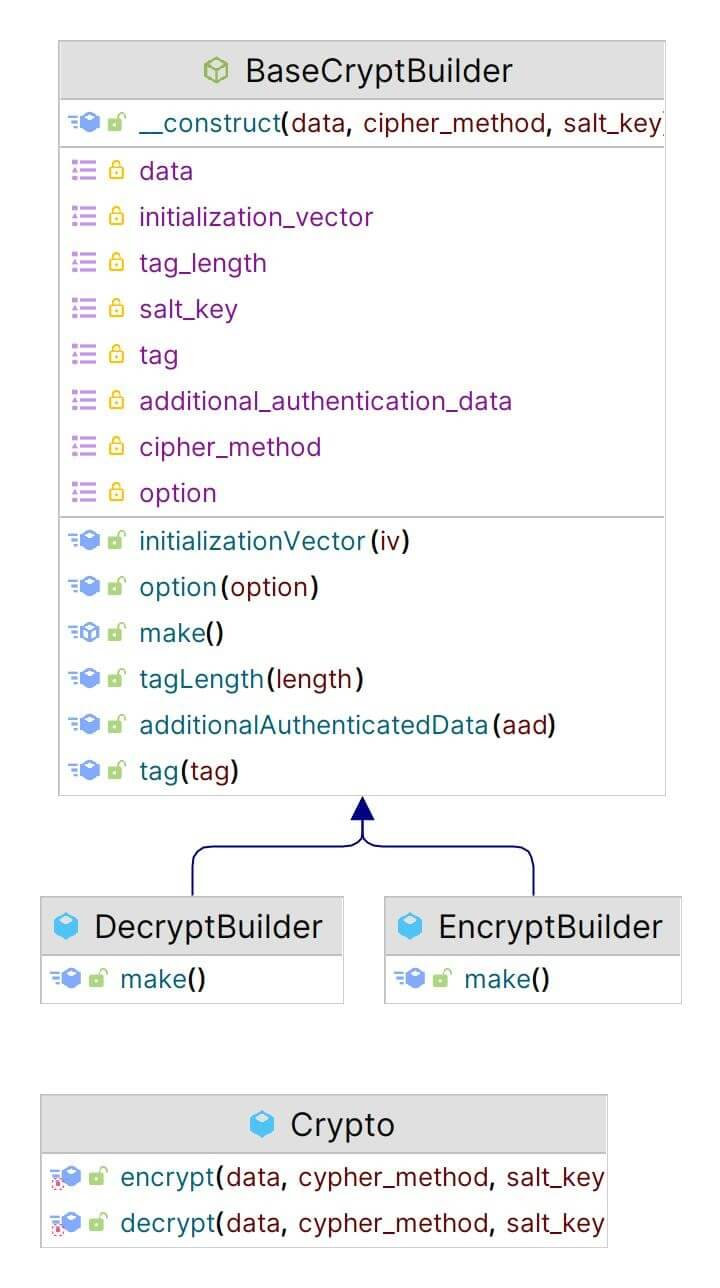
\includegraphics[width=0.4\linewidth]{figures/11_cryptography.jpg}
    \caption{Classes de criptografia}
    \label{fig:11_cryptography}
\end{figure}

A figura \ref{fig:11_cryptography} agrupa as classes para realizar a encriptação e a decriptação de \textit{strings}.

 \begin{enumerate}
     \item \textbf{BaseCryptBuilder.} Classe abstrata base para as classes subsequentes EncryptBuilder e DecryptBuilder.
     \item \textbf{DecryptBuilder.} Classe responsável por realizar a decriptação.
     \item \textbf{EncryptBuilder.} Classe responsável por realizar a encriptação.
     \item \textbf{Crypto.} \textit{Facade} para acessar as classes \textit{builders} de encriptação e decriptação.
 \end{enumerate}

  \section{Abstrações globais}

\begin{figure}[H]
    \centering
    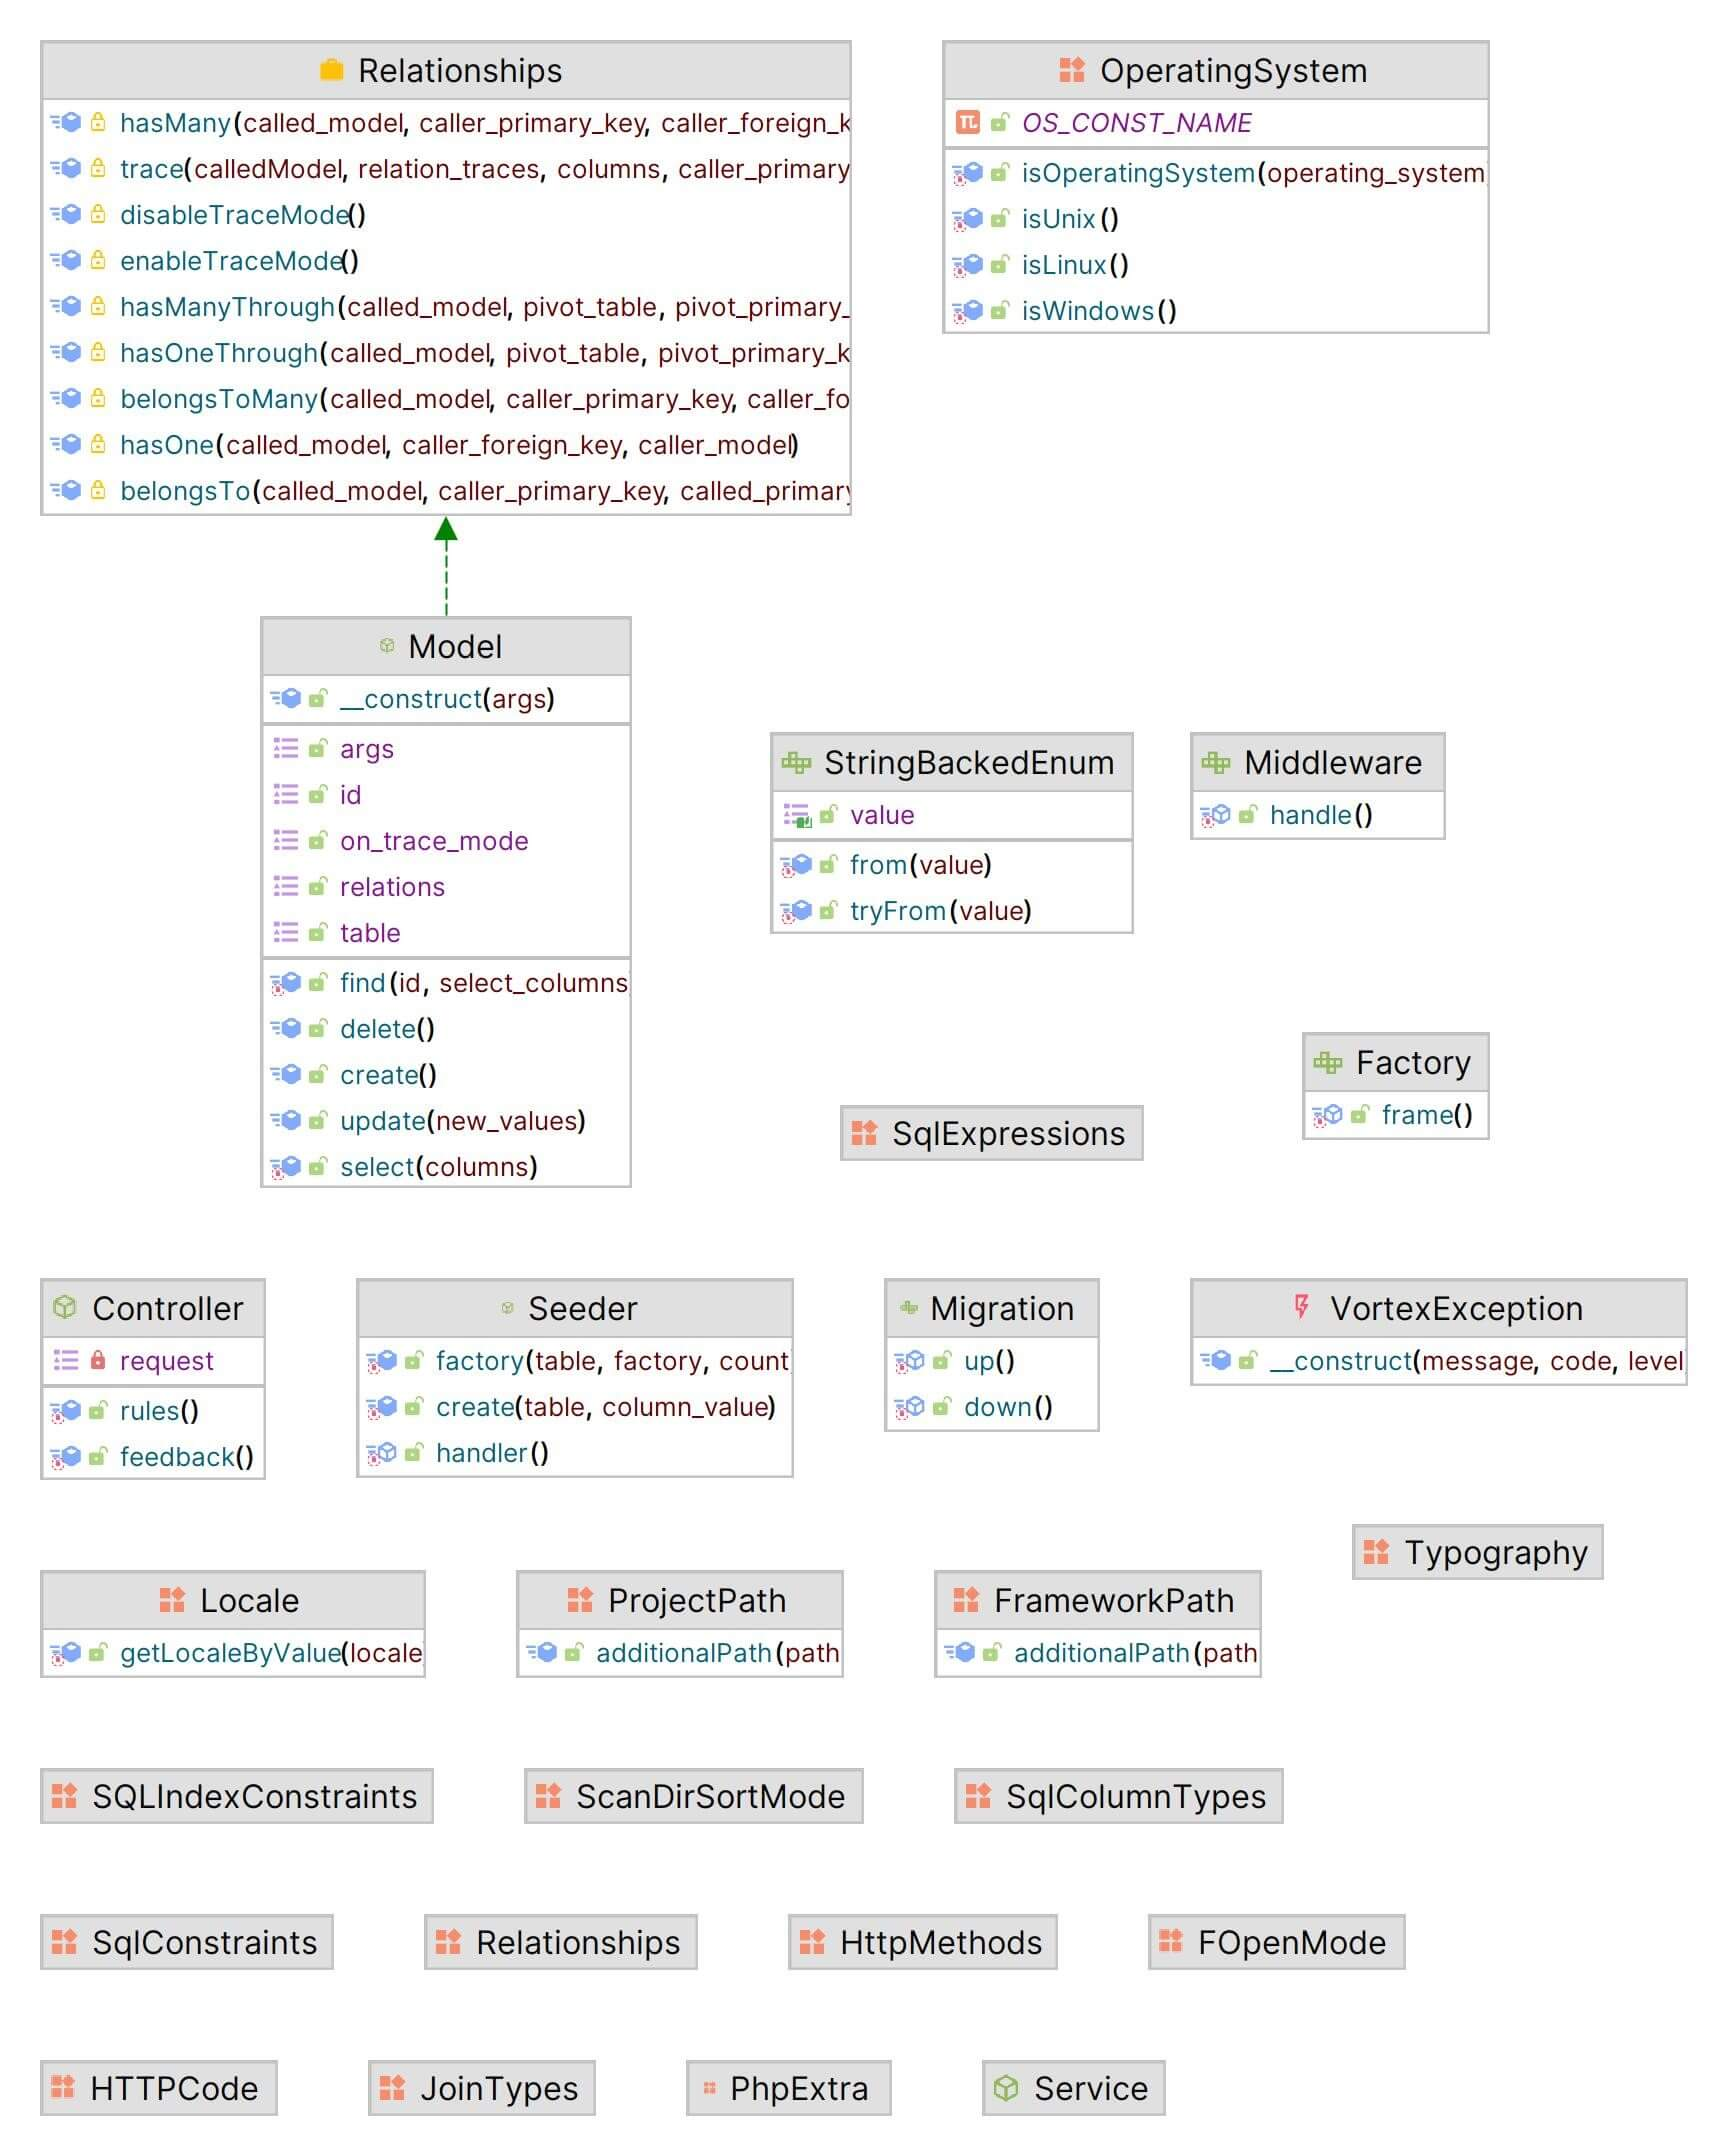
\includegraphics[width=0.7\linewidth]{figures/12_abstractions.jpg}
    \caption{Classes abstratas globais}
    \label{fig:12_abstractions}
\end{figure}

Na figura \ref{fig:12_abstractions} temos as classes abstratas e suas \textit{traits} no contexto global da aplicação. São classes que tem ligação com diversas partes da aplicação, ou o extremo oposto, funcionando singularmente. 

 \begin{enumerate}
     \item \textbf{Controller.} Classe abstrata com as funcionalidades para criação de novas controladoras.
     \item \textbf{Seeder.} Abstração que serve de base para classes semente, que são responsáveis por fazer inserções programadas na base de dados.
     \item \textbf{Migration.} Interface que serve de base para criação de novas migrações que são responsáveis por inserções pontuais na base de dados.
     \item \textbf{VortexException.} Classe para criação de novas exceções integradas com o \textit{framework}.
     \item \textbf{Factory.} A interface \textit{factory} serve de molde para novas classes que servem de \textit{frame} para geração de dados aleatórios na inserção massiva de dados na base de dados.
     \item \textbf{Model.} Classe abstrata que serve de base para interação com o ORM.
     \item \textbf{Relationships.} \textit{Trait} que possui os métodos de integração com o ORM, é utilizada pela classe Model.
     \item \textbf{Middleware.} Interface base para criação de \textit{middlewares} que são chamados antes dos \textit{controllers}.
 \end{enumerate}

  \section{\textit{Trigger}, \textit{View}, \textit{Index} e Procedures}

\begin{figure}[H]
    \centering
    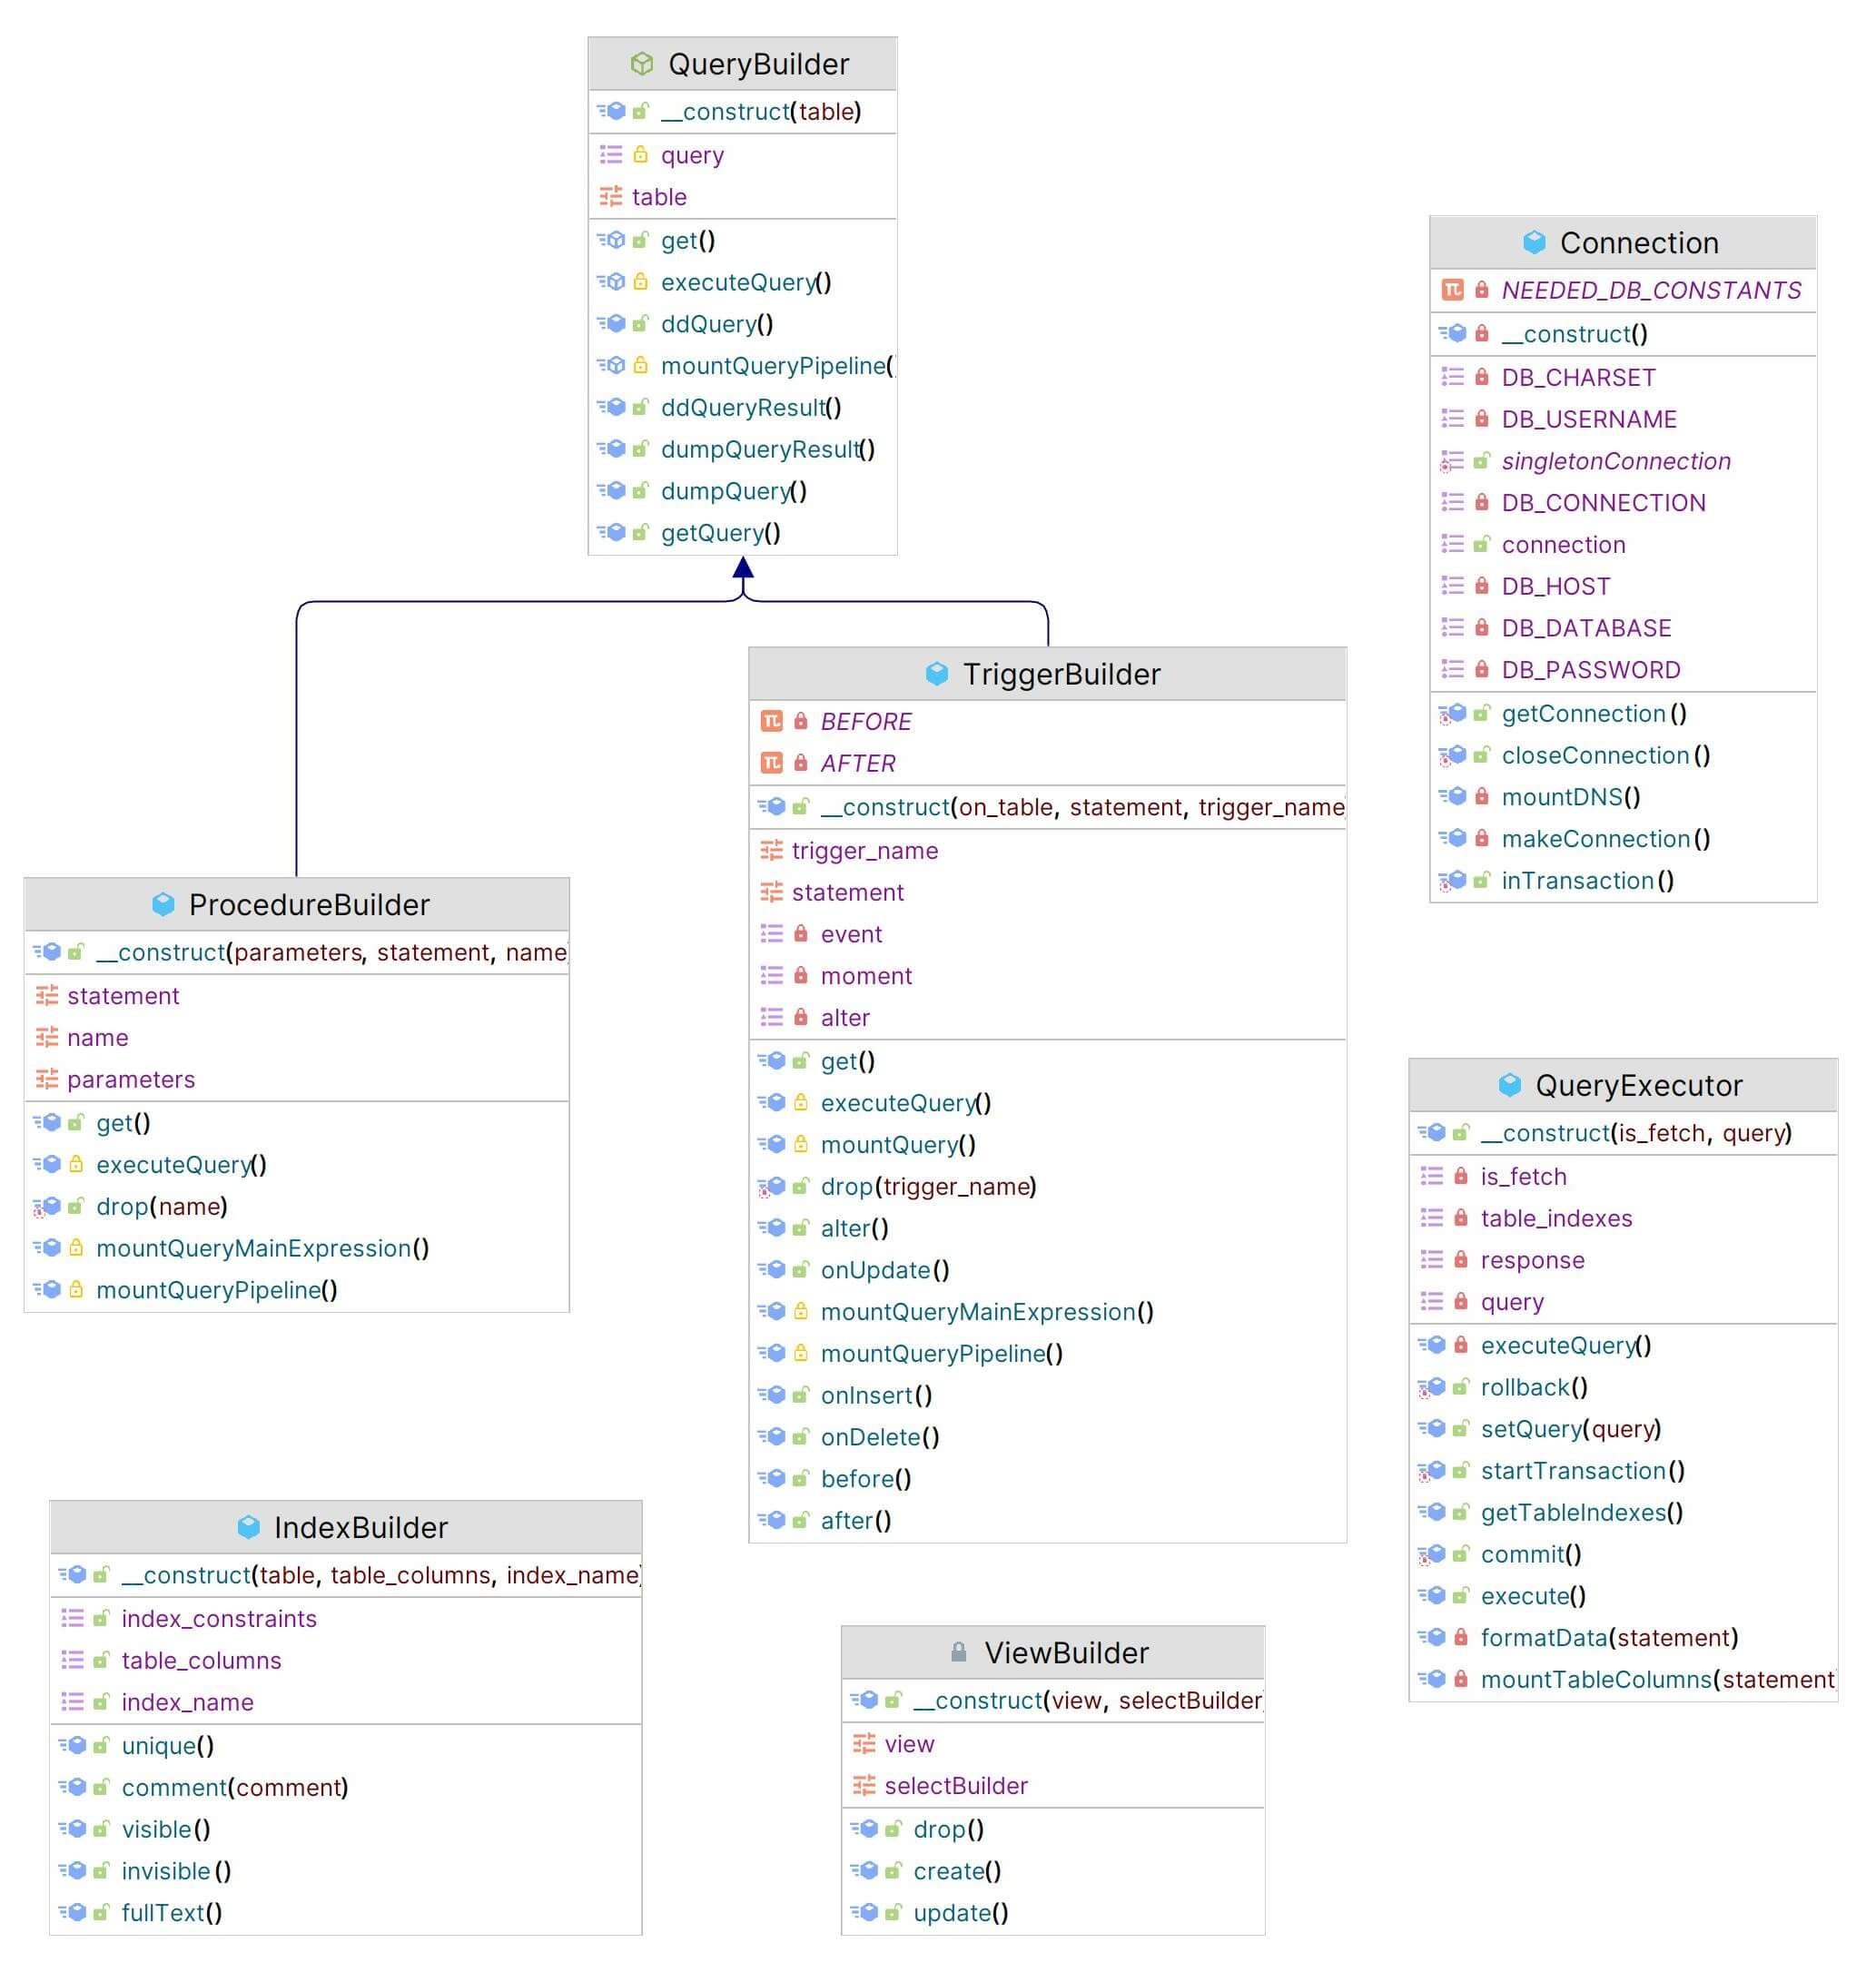
\includegraphics[width=0.7\linewidth]{figures/13_trigger_procedure_view.jpg}
    \caption{\textit{Builders} para \textit{Trigger}, \textit{View}, \textit{Index} e \textit{Procedures}}
    \label{fig:13_trigger_procedure_view}
\end{figure}

A figura \ref{fig:13_trigger_procedure_view} inclui as classes \textit{builders} para montagem de migrações que deveram criar \textit{Trigger}, \textit{View}, \textit{Index} e \textit{Procedures}. Além de classes responsáveis por realizar a conexão com a base de dados.

 \begin{enumerate}
     \item \textbf{QueryBuilder.} Classe abstrata responsável por servir de base para classes \textit{builders} do ORM.
     \item \textbf{TriggerBuilder.} \textit{Builder} para montagem de migrações de \textit{triggers};
     \item \textbf{ProcedureBuilder.} \textit{Builder} para criação de migrações de \textit{procedures}.
     \item \textbf{IndexBuilder.} \textit{Builder} para gerar indexes em migrações de criação de tabelas.
     \item \textbf{ViewBuilder.} \textit{Builder} para criação de migrações de \textit{views}.
     \item \textbf{Connection.} \textit{Singleton} para realizar a conexão com a base de dados.
     \item \textbf{QueryExecutor.} Classe final para execução de \textit{querys} com a base de dados. Esta é a única classe que utiliza a classe de conexão.
 \end{enumerate}

  \section{Classes de relacionamentos}

\begin{figure}[H]
    \centering
    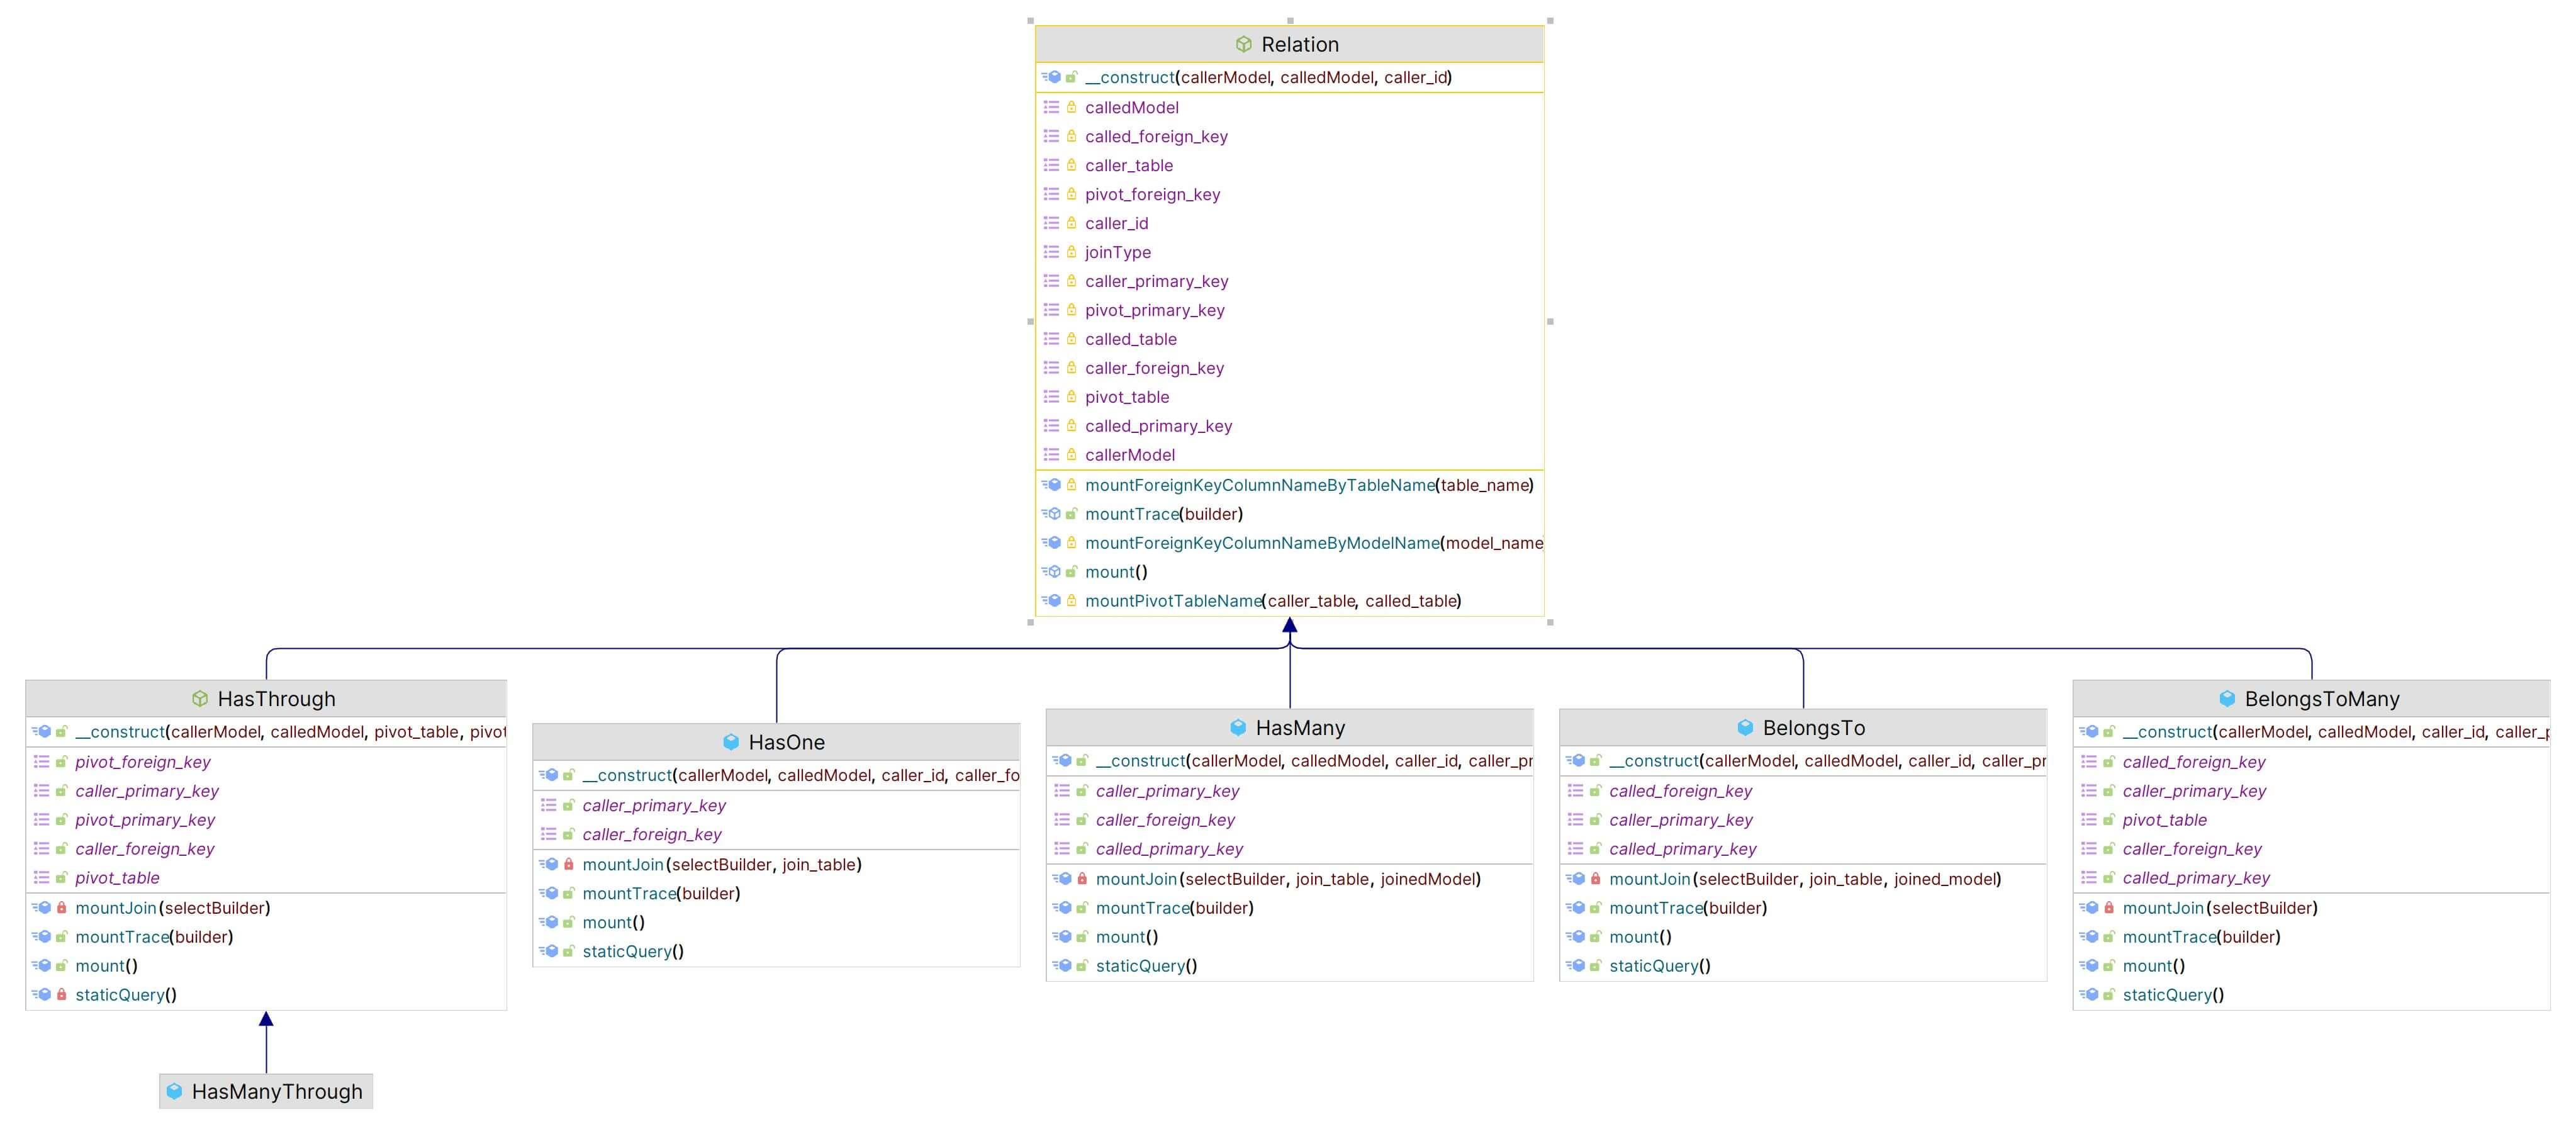
\includegraphics[width=0.9\linewidth]{figures/14_relationships.jpg}
    \caption{\textit{Builders} para \textit{Trigger}, \textit{View}, \textit{Index} e \textit{Procedures}}
    \label{fig:14_relationships}
\end{figure}

Na figura \ref{fig:14_relationships} temos as classes que representam os relacionamentos que serão integrados na classe modelo que serão integrados pelo ORM.

 \begin{enumerate}
     \item \textbf{Relation.} Classe abstrata para criação de relacionamentos.
     \item \textbf{\{Demais classes\}.} As demais classes do diagrama \ref{fig:14_relationships} representam relacionamentos e possuem a mesma estrutura de métodos e atributos, porém os mesmos espcificos para se adequar a cada classe. 
 \end{enumerate}

  \section{\textit{Select builder}}
  \label{sec:select_builder}

\begin{figure}[H]
    \centering
    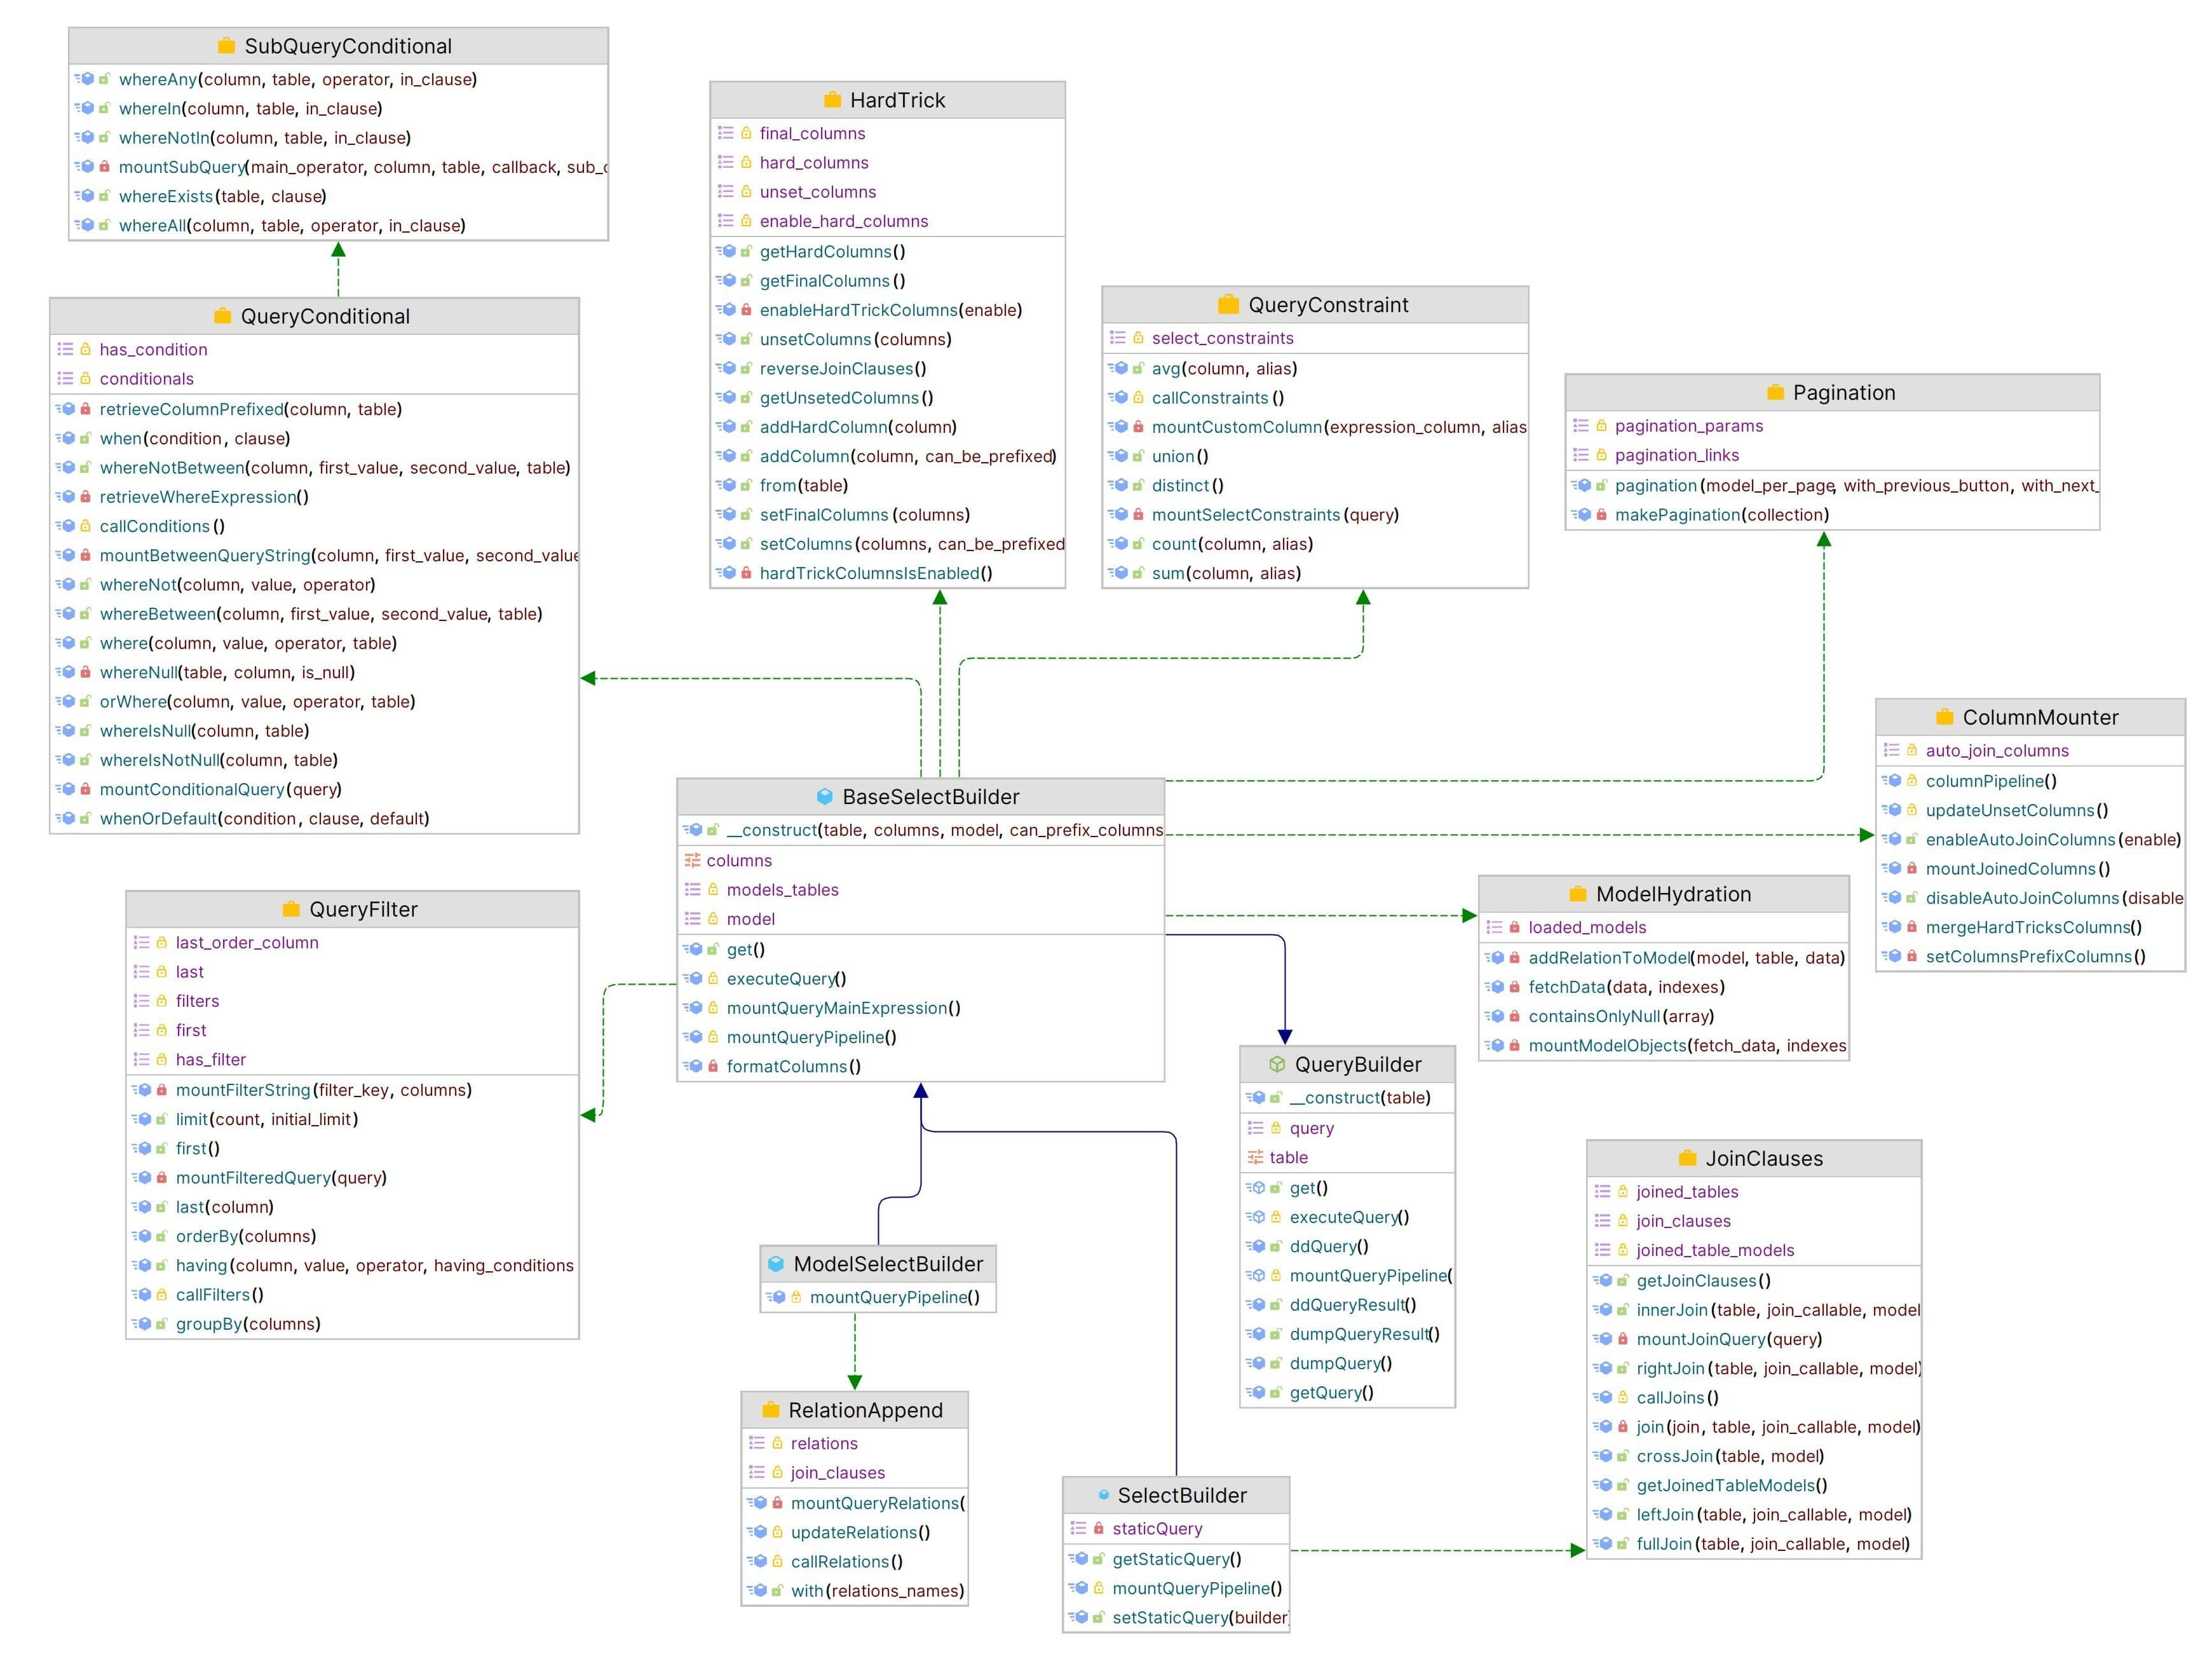
\includegraphics[width=0.9\linewidth]{figures/15_select_builder.jpg}
    \caption{Classes construtoras para montagem de consultas}
    \label{fig:15_select_builder}
\end{figure}

Na figura \ref{fig:15_select_builder} tem-se as classes que integram a lógica de criação de consultas e a hidratação de resultados de \textit{queries}.

 \begin{enumerate}
     \item \textbf{BaseSelectBuilder.} Classe abstrata para dar fundamento aos \textit{buiders} que fazem a construção de consultas.
     \item \textbf{SelectBuilder.} Este \textit{builder} é responsável por criar as consultas sem a integração mandatória de classes modelos. Representa a integração mais direta com a linguagem SQL.
     \item \textbf{ModelSelectBuilder.} Classe abstrata para realizar consultas integradas com modelos.
     \item \textbf{QueryFilter.} \textit{Trait} com métodos para abstrair os filtros da linguagem SQL.
     \item \textbf{QueryConditional.} \textit{Trait} com métodos para abstrair as clausulas condicionais do SQL.
     \item \textbf{SubQueryConditional.} \textit{Trait} com métodos condicionais que possibilitam a construção de \textit{subqueries}.
     \item \textbf{HardTrick.} \textit{Trait} com métodos para alterações absolutas em consultas.
     \item \textbf{QUeryConstraint.} \textit{Trait} com métodos para abstrair as regras da linguagem SQL, como \textit{sum(), count()}, entre outros.
     \item \textbf{Pagination.} Classe que realiza a construção da lógica de paginação em consultas. Possui integração com HTML.
     \item \textbf{ColumnMounter.} \textit{Trait} que implementa o \textit{pipeline} de montagem das colunas e suas dependências.
     \item \textbf{ModelHydration.} \textit{Trait} que ''hidrata'' as consultas integradas com modelos, permitindo a criação de modelos a partir de resultados de \textit{queries}.
     \item \textbf{JoinClauses.} \textit{Trait} com métodos para abstrair os filtros da linguagem SQL.
     \item \textbf{RelationAppend.} \textit{Trait} que direciona os relacionamentos em objetos modelos. 
 \end{enumerate}

  \section{\textit{Update builder}}

\begin{figure}[H]
    \centering
    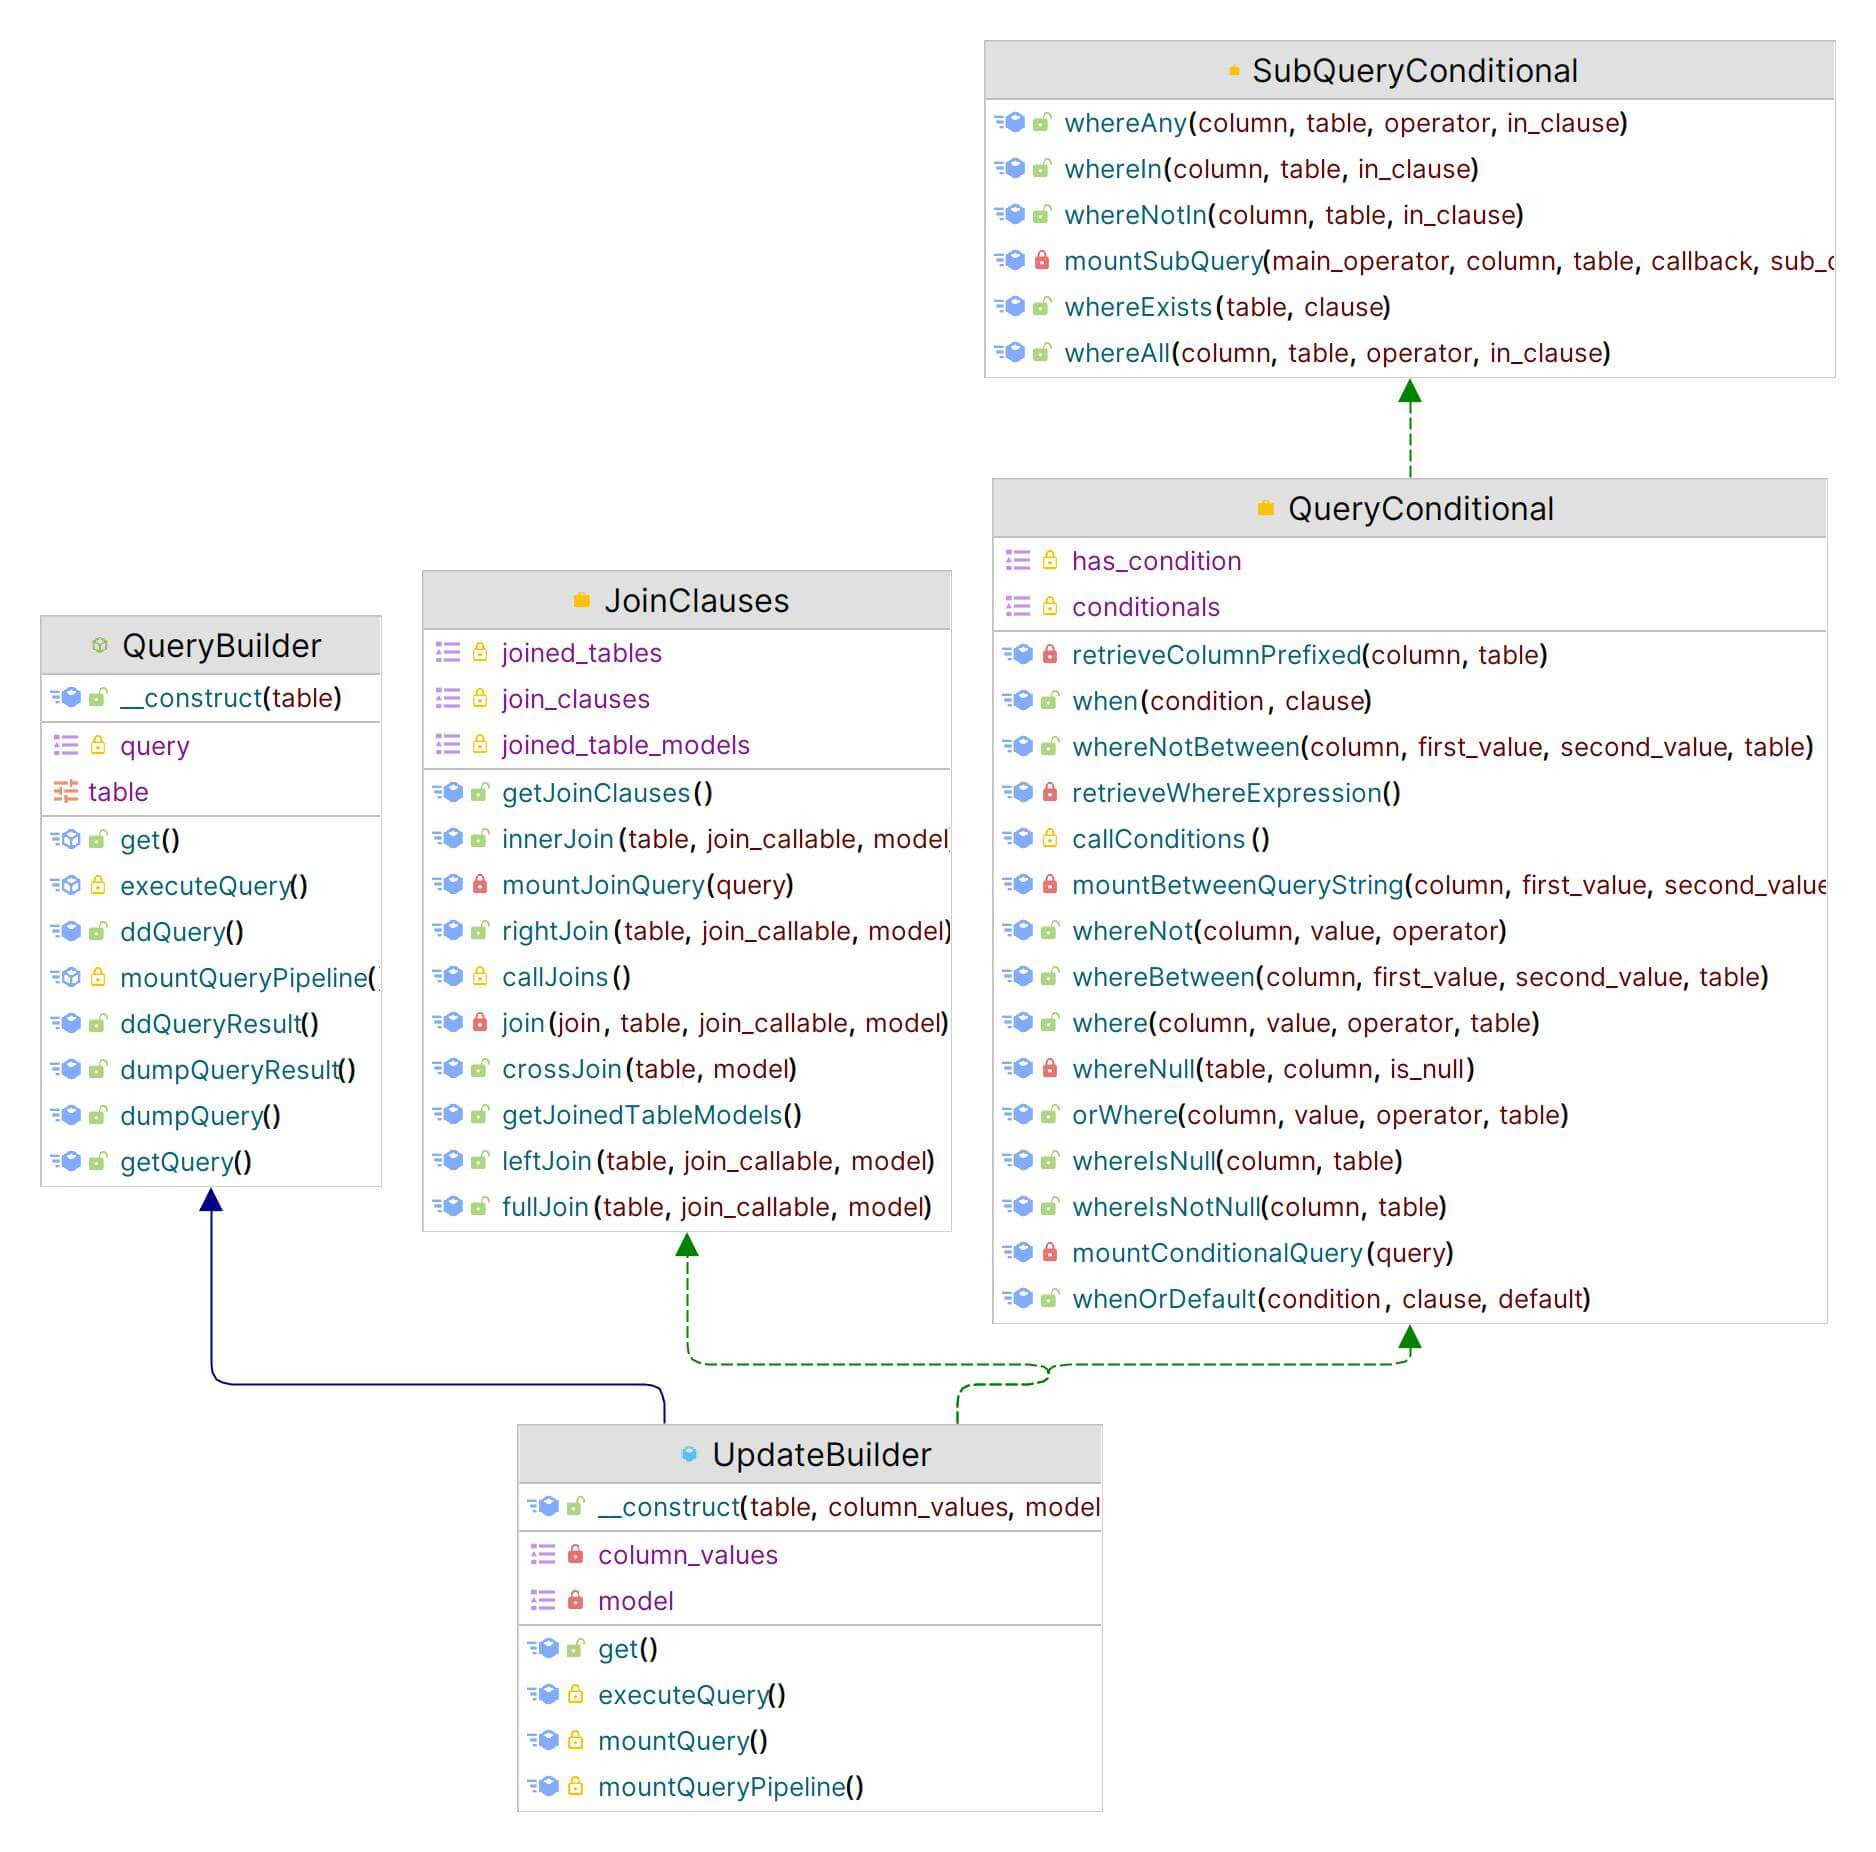
\includegraphics[width=0.7\linewidth]{figures/16_update_builder.jpg}
    \caption{Classe construtora para montagem de \textit{updates}}
    \label{fig:16_update_builder}
\end{figure}

A figura \ref{fig:16_update_builder} possui o conjunto de classes que formam a lógica de construção de consultas de atualização. A classe \textit{UpdateBuilder} é responsável por montar a consulta final, as demais \textit{traits} já foram descritas anteriormente na sessão \ref{sec:select_builder}.

 \begin{enumerate}
     \item \textbf{UpdateBuilder.} Classe que realiza a montagem de consultas \textit{update} no ORM do Vortex. 
 \end{enumerate}

   \section{\textit{Delete builder}}

\begin{figure}[H]
    \centering
    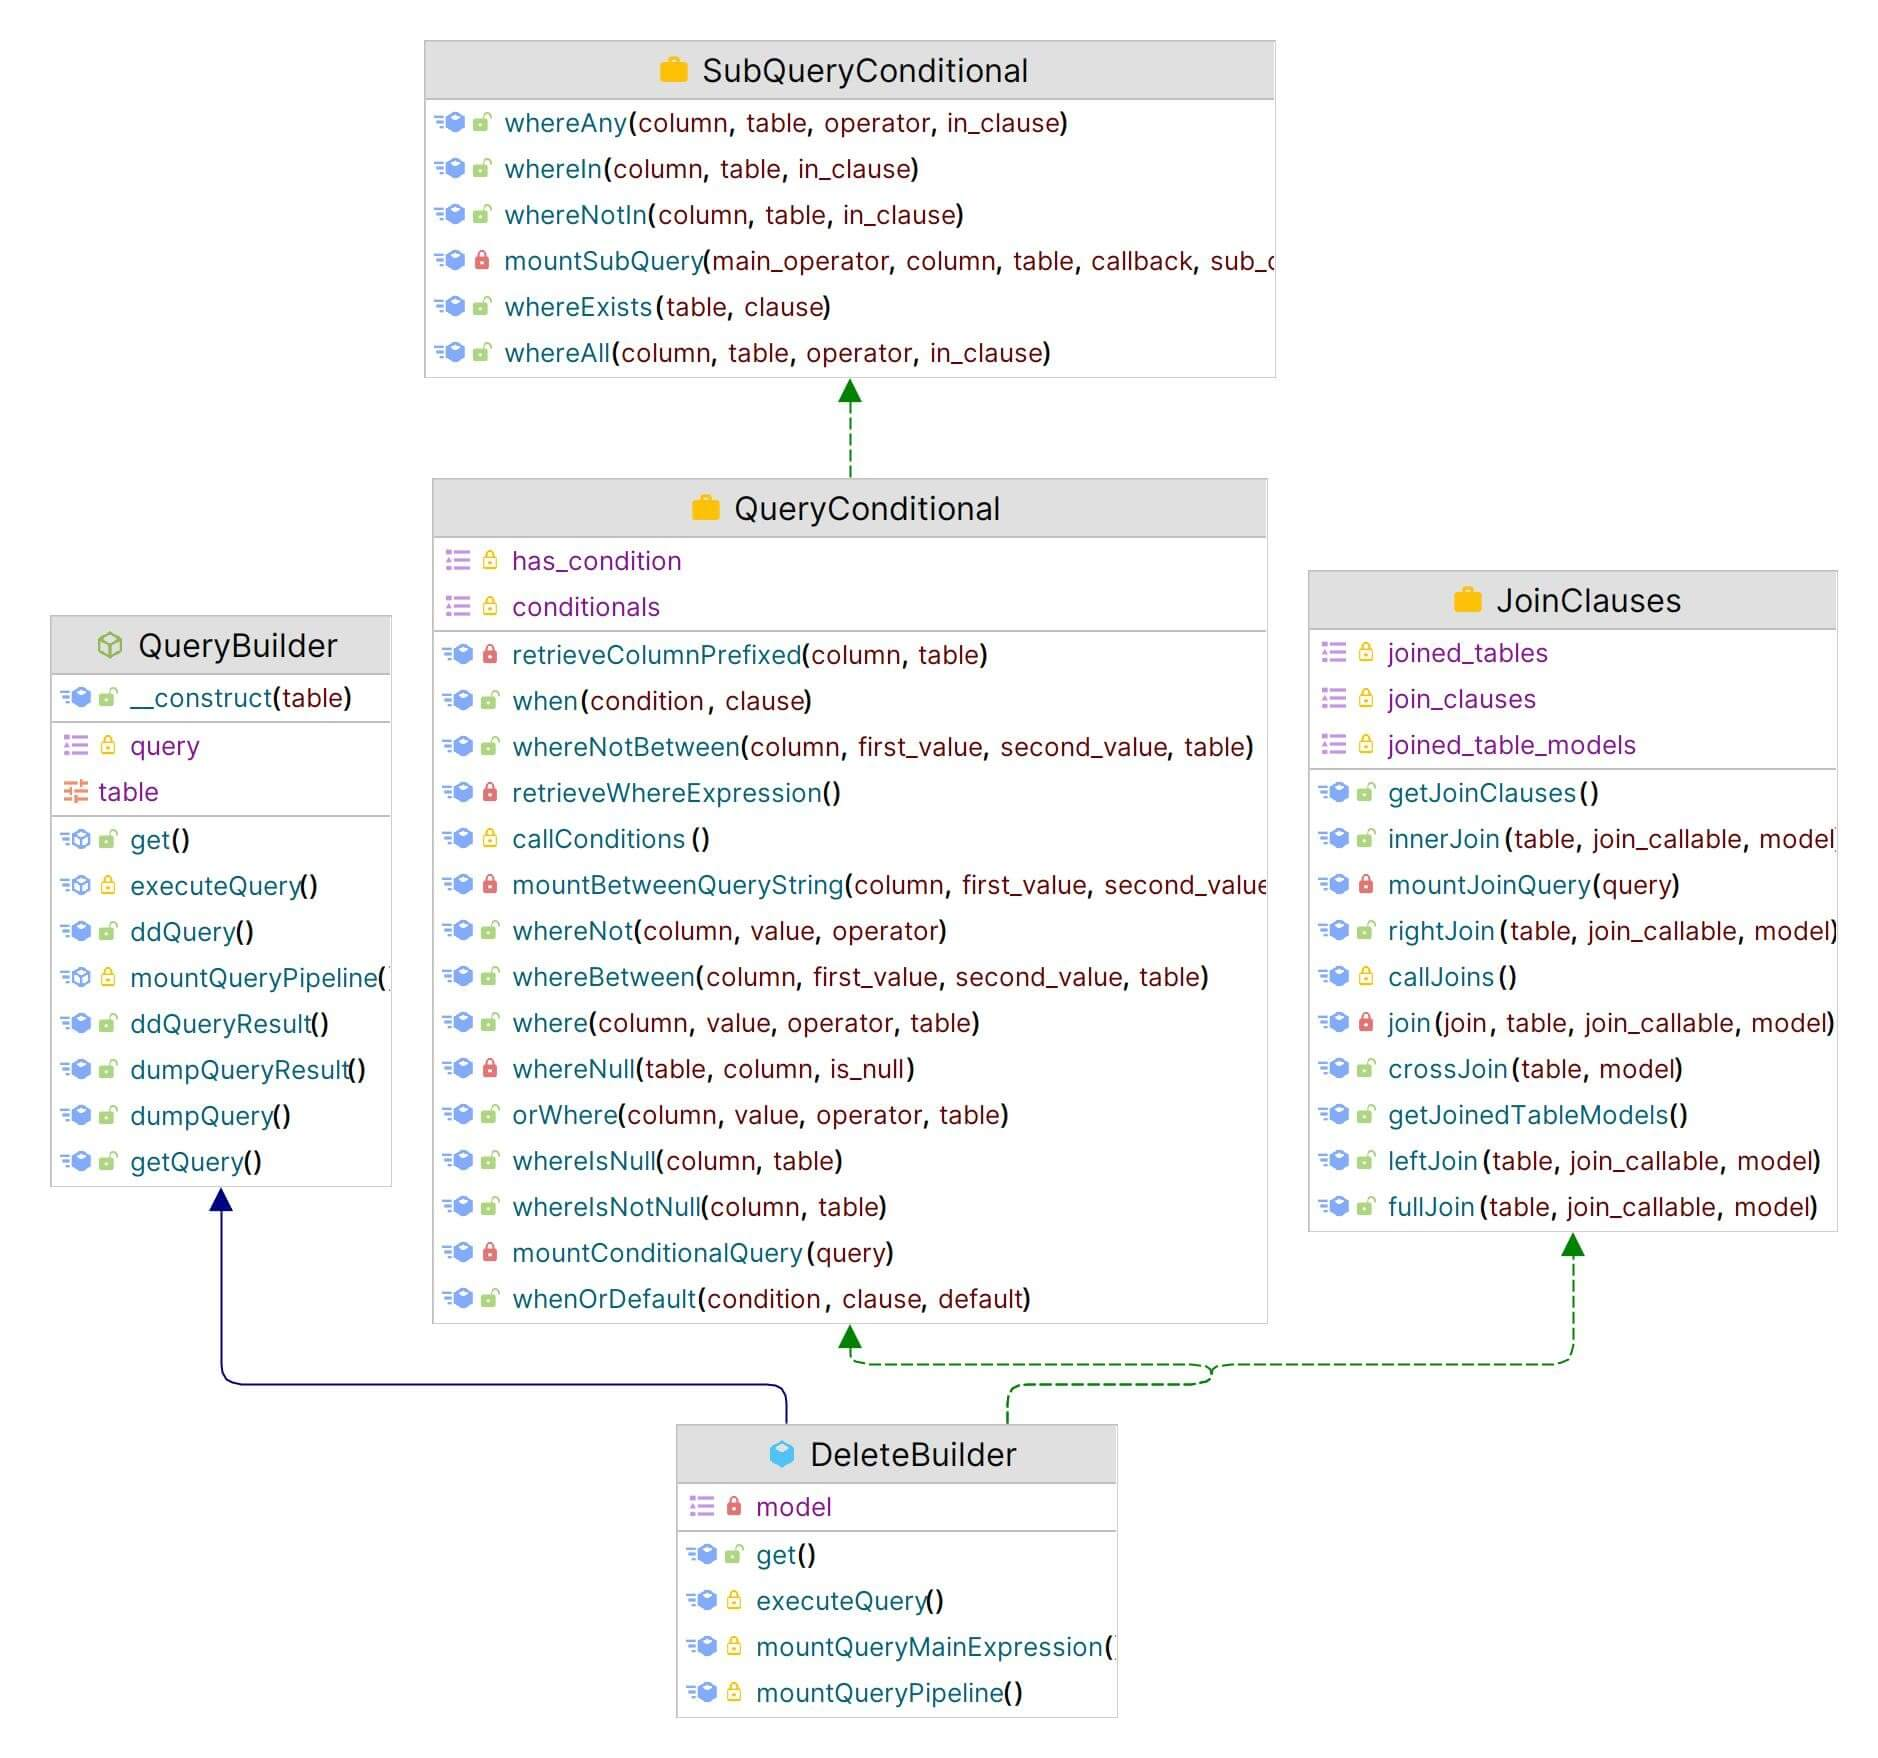
\includegraphics[width=0.7\linewidth]{figures/17_delete_builder.jpg}
    \caption{Classe construtora para montagem de \textit{deletes}}
    \label{fig:17_delete_builder}
\end{figure}

A figura \ref{fig:17_delete_builder} contém as classes que permitem a exclusão de recursos da base de dados. A classe \textit{DeleteBuilder} monta a \textit{query} que realiza a exclusão, as demais \textit{traits} já foram descritas anteriormente na sessão \ref{sec:select_builder}.

 \begin{enumerate}
     \item \textbf{DeleteBuilder.} \textit{Builder} que implementa a lógica de exclusão de recursos, tanto a partir de modelos quanto por \textit{queries} ''livres''.
 \end{enumerate}

\section{\textit{Insert builder}}

\begin{figure}[H]
    \centering
    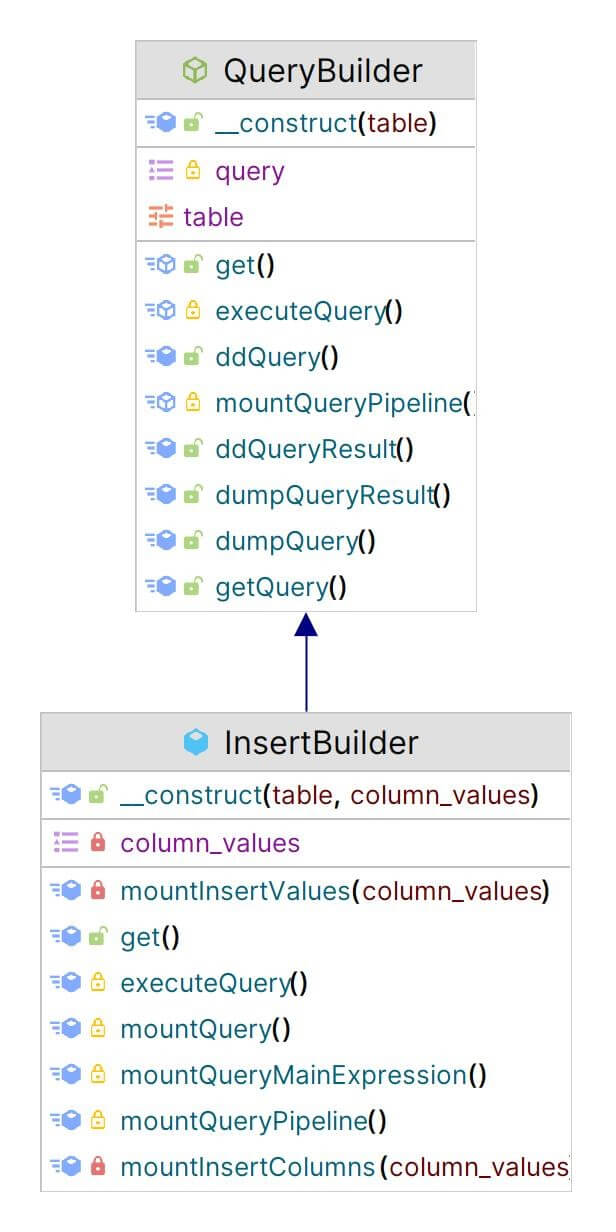
\includegraphics[width=0.4\linewidth]{figures/18_insert_builder.jpg}
    \caption{Classe construtora para montagem de \textit{inserts}}
    \label{fig:18_insert_builder}
\end{figure}

A figura \ref{fig:18_insert_builder} contém as classes que permitem a exinserção de recursos da base de dados. A classe \textit{InsertBuilder} monta a \textit{query} que realiza a inserção, as demais \textit{traits} já foram descritas anteriormente na sessão \ref{sec:select_builder}.

 \begin{enumerate}
     \item \textbf{InsertBuilder.} \textit{Builder} que implementa a lógica de inserção de recursos, tanto a partir de modelos quanto por \textit{queries} ''livres''.
 \end{enumerate}

 \section{\textit{Table builder}}

\begin{figure}[H]
    \centering
    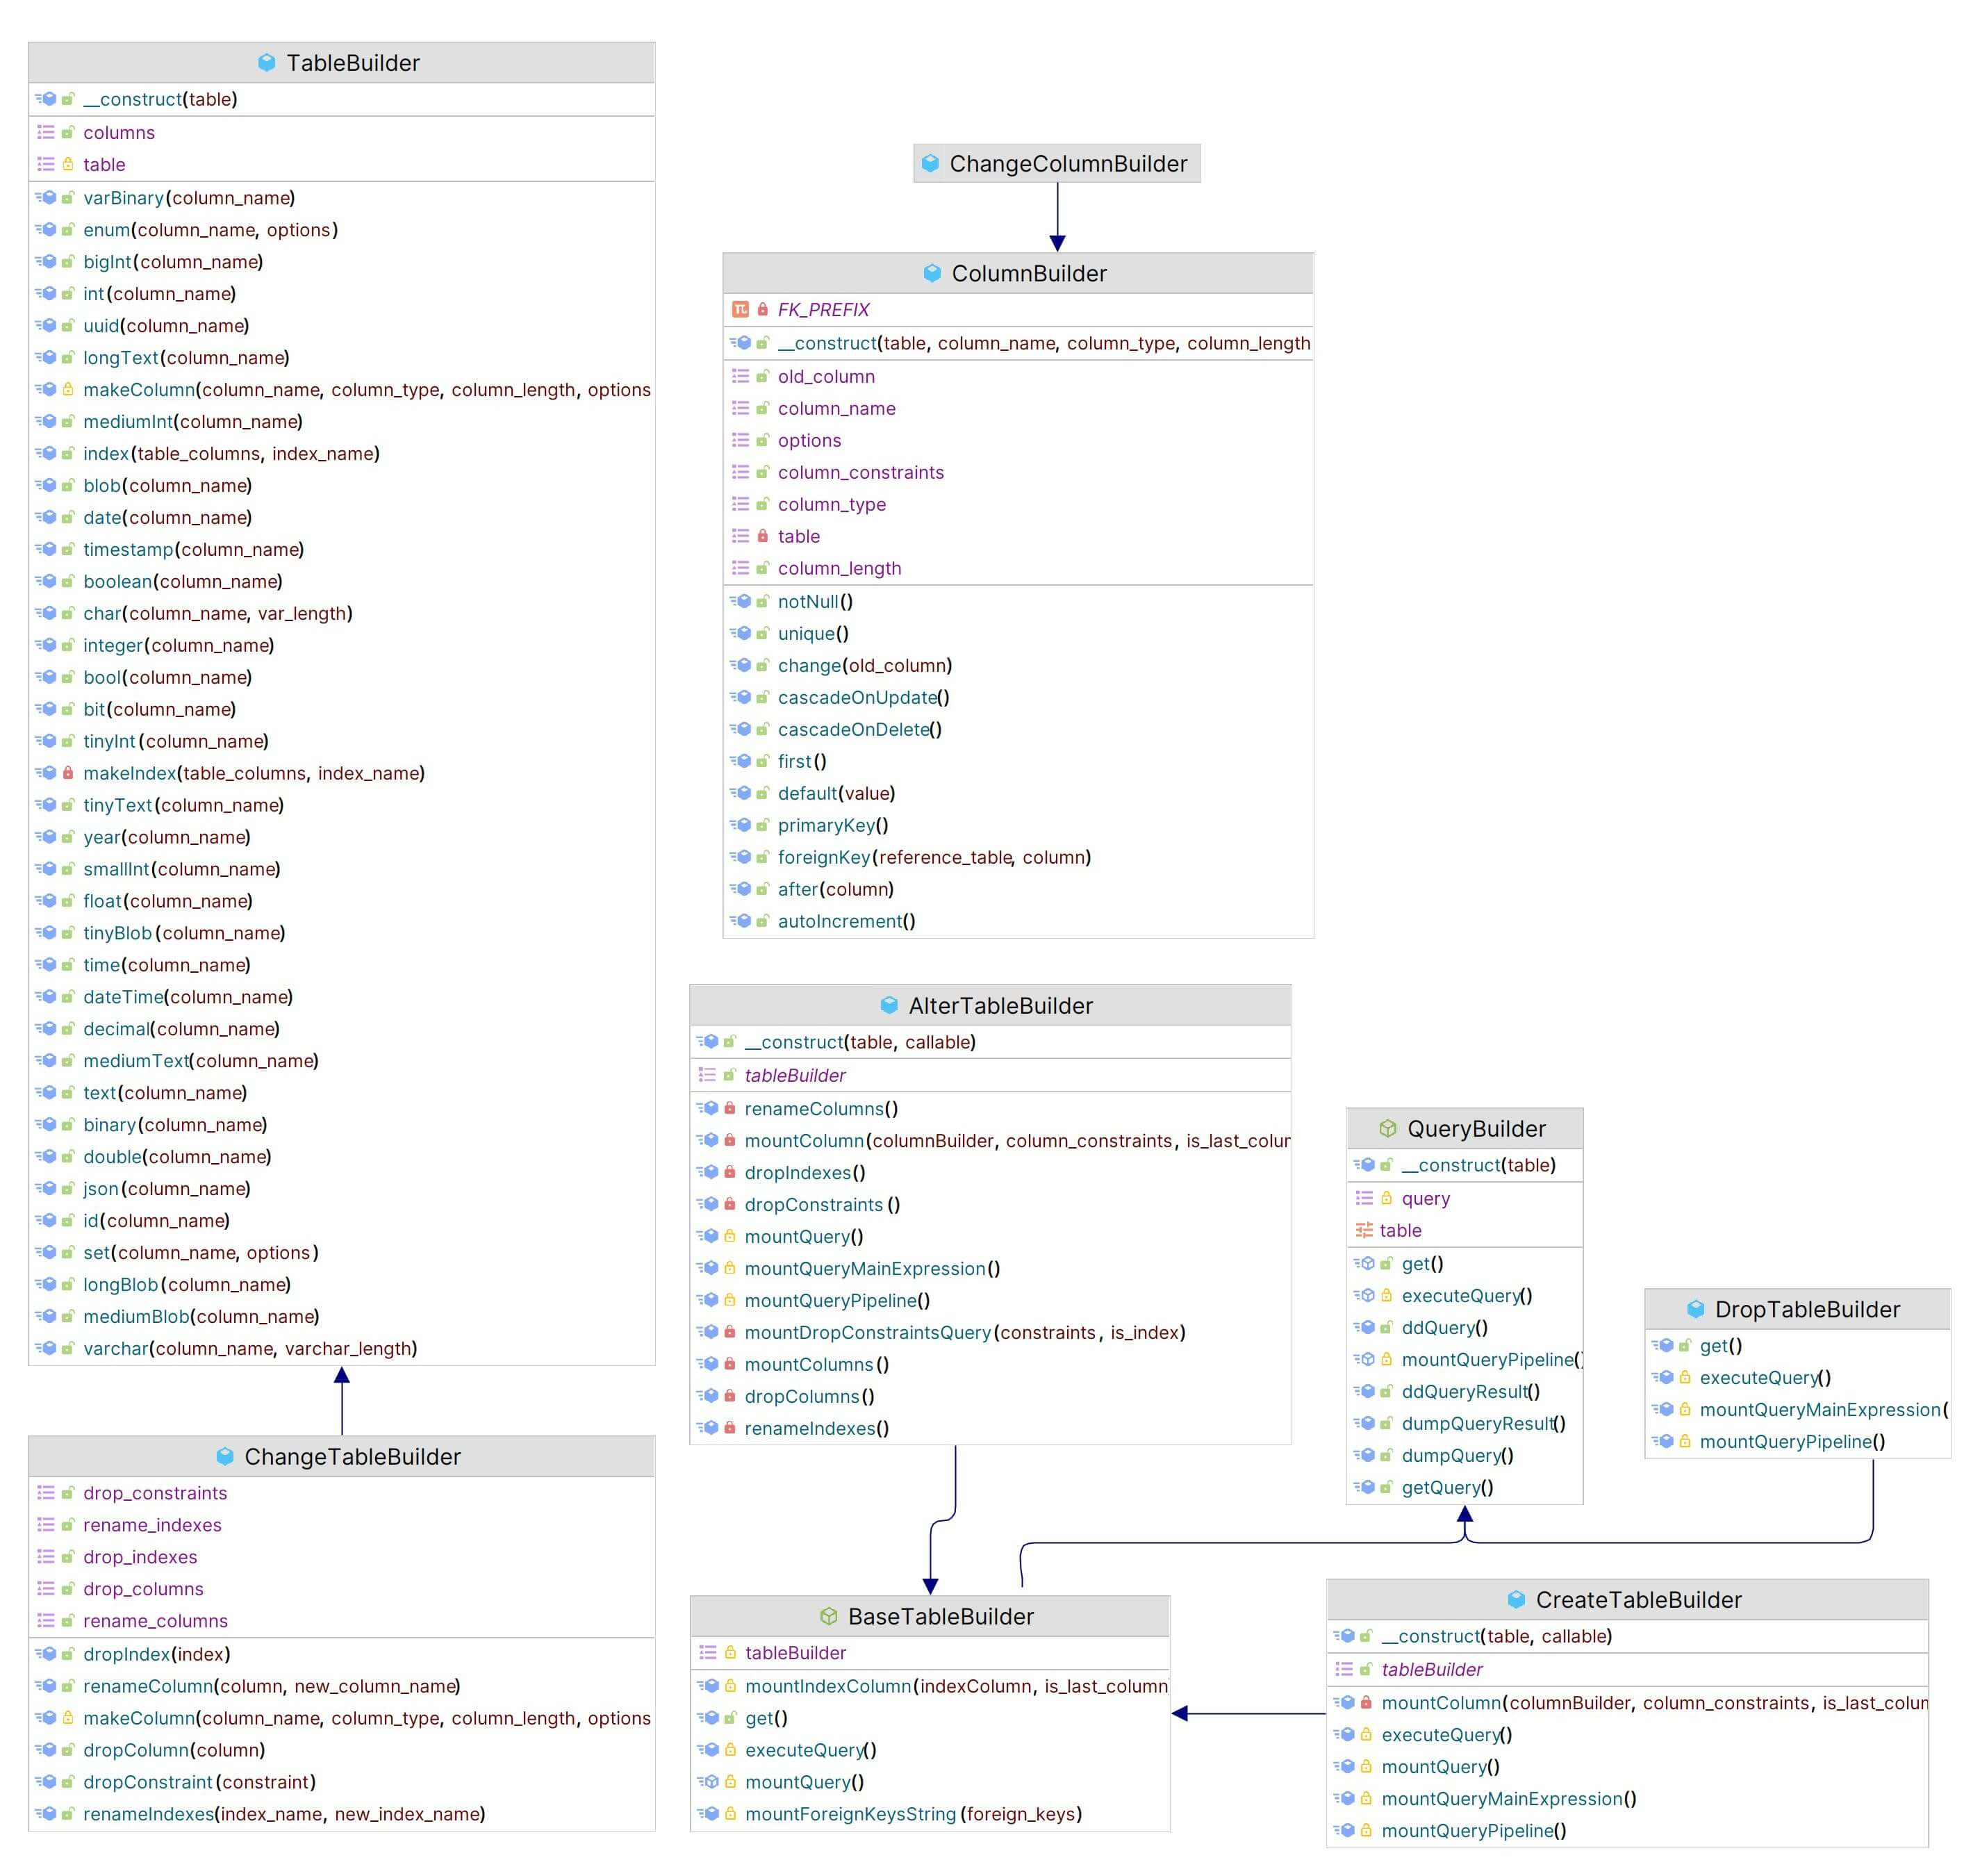
\includegraphics[width=0.9\linewidth]{figures/19_table_builder.jpg}
    \caption{Classe construtora para montagem de tabelas em migrações}
    \label{fig:19_table_builder}
\end{figure}

A figura \ref{fig:19_table_builder} contém as classes que permitem criação de tabelas em classes de migração, versionando suas colunas, \textit{constraints} e toda a estrutura das mesmas.

 \begin{enumerate}
     \item \textbf{TableBuilder.} Classe que gera o objeto com a representação da tabela que será criada ao executar a migração.
     \item \textbf{ChangeTableBuilder.} Classe que permite alterar a estrutura de colunas e indices de determinada tabela.
     \item \textbf{BaseTableBuilder.} Classe abstrata que serve de base para os \textit{builders} de tabelas.
     \item \textbf{AlterTableBuilder.} Classe que altera a estrutura da tabela, podendo deletar a tabela, renomear e manejar índices.
     \item \textbf{ColumnBuilder.} \textit{Builder} que gera o objeto utilizado pela classe Table para criação de colunas de tabelas.
     \item \textbf{CreateTableBuilder.} Classe utilizada para criação de tabelas em migrações.
     \item \textbf{DropTableBuilder.} \textit{Builder} para exclusão de tabelas.
     \item \textbf{ChangeColumnBuilder.} \textit{Builder} para alteração da estrutura de colunas de determinada tabela.
 \end{enumerate}